\documentclass[10pt,numbers]{sigplanconf}
%\documentclass[10pt,twocolumn]{article}
\usepackage{times}
\usepackage{url}                  % format URLs
\usepackage[colorlinks=true,allcolors=blue,breaklinks,draft=false]{hyperref}   % hyperlinks, including DOIs and URLs in bibliography
\usepackage{amsmath}
\usepackage{xspace}
\usepackage{algorithm}
\usepackage[noend]{algpseudocode}
\usepackage{subcaption}
\usepackage{xcolor}
%\usepackage[pdftex]{graphicx}
\usepackage{tikz}
\usepackage{arydshln}
\usepackage{acmcopyright}


\usepackage{pifont}
\usepackage{amssymb}

%\usepackage{titlesec}
\usepackage{multicol}

\usepackage{pgfplots}

%\usepackage[letterpaper,margin=0.75in,top=1in,bottom=1in]{geometry}


\definecolor{blues1}{RGB}{198, 219, 239}
\definecolor{blues2}{RGB}{158, 202, 225}
\definecolor{blues3}{RGB}{107, 174, 214}
\definecolor{blues4}{RGB}{49, 130, 189}
\definecolor{blues5}{RGB}{8, 81, 156}
\definecolor{antiquefuchsia}{rgb}{0.57, 0.36, 0.51}
\definecolor{asparagus}{rgb}{0.53, 0.66, 0.42}
\definecolor{darkspringgreen}{rgb}{0.09, 0.45, 0.27}
\definecolor{darkslategray}{rgb}{0.18, 0.31, 0.31}
\definecolor{coralred}{rgb}{1.0, 0.25, 0.25}

\pgfplotsset{mystyle/.style={%
        width=0.35\textwidth,
        xmin=1,xmax=32,
        enlargelimits=true,
	ymajorgrids=true,
        grid=major,
        grid style={dashed, gray!30},
        ylabel style={align=center, font=\small},
        xlabel style={align=center, font=\small},
        xtick={2,4,8,16,32}, 
         x tick label style={font=\tiny},
         y tick label style={font=\tiny},
        scaled y ticks=base 10:-6,
        ytick scale label code/.code={},
        title style={font=\small},
      	yticklabel={\pgfmathprintnumber{\tick}}
}}

\pgfplotsset{rangestyle/.style={%
        width=0.35\textwidth,
        enlargelimits=true,
	ymajorgrids=true,
        grid=major,
        grid style={dashed, gray!30},
        ylabel style={align=center, font=\small},
        xlabel style={align=center, font=\small},
        xticklabels={2, 8, 32, 128, 512, 2K, 8K, 32K},
        xtick={100,120,144,172,207,249,299,358},
        scaled y ticks=base 10:-6,
        ytick scale label code/.code={},
        x axis label/.style={font=\tiny},
        x tick label style={font=\tiny},
        y tick label style={font=\tiny},
        title style={font=\small},
    	yticklabel={\pgfmathprintnumber{\tick}}
}}

\pgfplotsset{mystyle16/.style={%
        width=0.35\textwidth,
        xmin=1,xmax=16,
        enlargelimits=true,
	ymajorgrids=true,
        grid=major,
        grid style={dashed, gray!30},
        ylabel style={align=center, font=\small},
        xlabel style={align=center, font=\small},
        xtick={1,2,4,8,16}, 
         x tick label style={font=\tiny},
         y tick label style={font=\tiny},
        scaled y ticks=base 10:-6,
        ytick scale label code/.code={},    
        title style={font=\small},
    	yticklabel={\pgfmathprintnumber{\tick}}
}}

\pgfplotsset{memstyle16/.style={%
        width=0.35\textwidth,
        xmin=1,xmax=16,
        ymin=0,ymax=120,
        enlargelimits=true,
	ymajorgrids=true,
        grid=major,
        grid style={dashed, gray!30},
        ylabel style={align=center, font=\small},
        xlabel style={align=center, font=\small},
        xtick={1,2,4,8,16}, 
         x tick label style={font=\tiny},
         y tick label style={font=\tiny},
%        scaled y ticks=base 10:-6,
        ytick scale label code/.code={},    
        title style={font=\small},
    	yticklabel={\pgfmathprintnumber{\tick}}
}}

\pgfplotsset{chunksStyle/.style={%
        width=0.31\textwidth,
        xmin=1,xmax=55,
        enlargelimits=true,
	ymajorgrids=true,
        ylabel style={align=center},
        ytick scale label code/.code={},
       scaled x ticks=base 10:-1,
       scaled y ticks=base 10:-3,
       xtick scale label code/.code={},
       yticklabel={\pgfmathprintnumber{\tick}}
}}

\pgfplotsset{chunksUtilStyle/.style={%
        width=0.31\textwidth,
        xmin=1,xmax=55,
        enlargelimits=true,
	ymajorgrids=true,
        ylabel style={align=center},
       scaled y ticks=base 10:-3,
       ytick scale label code/.code={},
       scaled x ticks=base 10:-1,
       xtick scale label code/.code={},
       yticklabel={\pgfmathprintnumber{\tick}}
}}

\pgfplotsset{chunkLegendStyle/.style={%
	   %width=0.35\textwidth,
      % legend columns=-1,
	 legend columns=4,
	  legend entries={total, sorted , duplicates, nulls},
	  legend style={at={(1, 0)}, anchor=north east, font=\tiny},
	   legend to name=chunksDropHalfLegend,	  
}}

\pgfplotsset{chunkCountLegendStyle/.style={%
	   %width=0.35\textwidth,
      % legend columns=-1,
      	legend columns=2,
	legend entries={random, drop-half},
	legend style={font=\tiny},
	legend to name=chunksLegend,
}}


\pgfplotsset{sPut/.style={%
	   %width=0.35\textwidth,
       legend columns=-1,
	   legend entries={\kiwi, \kary ,\skiplist, \snaptree},
	   legend to name=sPutLegend,
}}

\pgfplotsset{putScan/.style={%
	   %width=0.35\textwidth,
       legend columns=-1,
	   legend entries={\kiwi, \kary ,\skiplist, \snaptree},
	   legend to name=putScanLegend,
}}

\pgfplotsset{scansOnly/.style={%
	   %width=0.35\textwidth,
       legend columns=-1,
	   legend entries={\kiwi, \kary, \skiplist (non-atomic), \snaptree},
	   legend to name=scansOnlyLegend,
}}

\pgfplotsset{unbalanced/.style={%
	   %width=0.35\textwidth,
       legend columns=-1,
	   legend entries={\kiwi, \kary ,\skiplist, \snaptree},
	   legend to name=singleKeyOpsLegend,
}}


\pgfplotsset{balanced/.style={%
	   %width=0.35\textwidth,
       legend columns=-1,
	   legend entries={\autoTreap, \danaAVL,\snaptree, \friendly,  \stmTreap,
	   \domTreap, \optAutoTreap}, legend to name=balancedLegened,
}}

\pgfplotsset{skiplist/.style={%
	   width=\textwidth,
       ymin=0,ymax=2800000,
       xtick={2,4,8,16,32}, 
       legend columns=-1,
	   legend entries={\autoSkiplist, \kary , \skiplist (not atomic), \stmSkiplist,
	   \domSkiplist}, legend to name=skiplistLegened,
}}

\pgfplotsset{skiplist1000/.style={%
	   width=\textwidth,
       ymin=0,ymax=150000,
       scaled y ticks=base 10:-3,
       xtick={2,4,8,16,32}, 
       legend columns=-1,
	   legend entries={\autoSkiplist, \kary, \skiplist (not atomic), \stmSkiplist,
	   \domSkiplist}, legend to name=skiplistLegened1000,
}}

\pgfplotsset{skiplistUpdate/.style={%
	   width=0.35\textwidth,
       ymin=0,ymax=5500000,
       xtick={1,2,4,8,16,32}, 
       legend columns=-1,
	   legend entries={\autoSkiplist, \kary , \skiplist (not atomic), \stmSkiplist,
	   \domSkiplist}, legend to name=skiplistLegenedUpdate,
}}

\newcommand{\remove}[1]{}

\hyphenation{skip-list}

%-------------Theorem Definitions ---------------%
\newtheorem{theorem}{Theorem}[section]
\newtheorem{lemma}[theorem]{Lemma}
\newtheorem{claim}[theorem]{Claim}
\newtheorem{observation}[theorem]{Observation}
\newtheorem{proposition}[theorem]{Proposition}
\newtheorem{corollary}[theorem]{Corollary}
\newtheorem{invariant}{Invariant}

%\newenvironment{proof}[1][Proof]{\begin{trivlist}
%\item[\hskip \labelsep {\bfseries #1}]}{\qedsymb\end{trivlist}}
\newenvironment{definition}[1][Definition]{\begin{trivlist}
\item[\hskip \labelsep {\bfseries #1}]}{\end{trivlist}}
\newenvironment{example}[1][Example]{\begin{trivlist}
\item[\hskip \labelsep {\bfseries #1}]}{\end{trivlist}}
\newenvironment{remark}[1][Remark]{\begin{trivlist}
\item[\hskip \labelsep {\bfseries #1}]}{\end{trivlist}}


%\newcommand{\qed}{\nobreak \ifvmode \relax \else
%      \ifdim\lastskip<1.5em \hskip-\lastskip
%      \hskip1.5em plus0em minus0.5em \fi \nobreak
%      \vrule height0.75em width0.5em depth0.25em\fi}
%\newcommand{\qedsymb}{\hfill{\rule{2mm}{2mm}}}


\newcommand{\codesize}{\footnotesize}
%--------------------------------------------------%

\newcommand{\code}[1]{\textsf{\fontsize{9.4}{11}\selectfont #1}}
\newcommand{\codeF}[1]{\textsf{#1}}
\newcommand{\readV}{\code{read\_version}\xspace}
\newcommand{\readSet}{\code{read\_set}\xspace}
\newcommand{\writeV}{\code{write\_version}\xspace}

\newcommand{\reqI}{\textbf{LPR1}\xspace}
\newcommand{\reqII}{\textbf{LPR2}\xspace}

%---------Evaluation Macros-----------------------%
\newcommand{\autoTree}{LR-Tree\xspace}
\newcommand{\autoTreap}{LR-Treap\xspace}
\newcommand{\optAutoTree}{Opt-LR-Tree\xspace}
\newcommand{\optAutoTreap}{Opt-LR-Treap\xspace}
\newcommand{\autoSkiplist}{LR-Skiplist\xspace}
\newcommand{\danaTree}{LO-Tree\xspace}
\newcommand{\danaAVL}{LO-AVL\xspace}
\newcommand{\bronson}{snap-tree\xspace}
\newcommand{\friendly}{CF-Tree\xspace}
\newcommand{\skiplist}{Java skiplist\xspace}
\newcommand{\kary}{k-ary tree\xspace}
\newcommand{\lockfreeTree}{LF-Tree\xspace}
\newcommand{\globalTree}{Global-Tree\xspace}
\newcommand{\globalTreap}{Global-Treap\xspace}
\newcommand{\domTree}{Lock-Tree\xspace}
\newcommand{\domTreap}{Lock-Treap\xspace}
\newcommand{\stmTree}{STM-Tree\xspace}
\newcommand{\stmTreap}{STM-Treap\xspace}
\newcommand{\stmSkiplist}{STM-Skiplist\xspace}
\newcommand{\domSkiplist}{Lock-Skiplist\xspace}
\newcommand{\getOP}{\textsc{get}\xspace}


%---------Comments -----------------------%
\newcommand{\Idit}[1]{{\color{red}{[\textbf{Idit:} #1 ]}}}
\newcommand{\guy}[1]{{\color{red}{[\textbf{guy:} #1 ]}}}
\newcommand{\eshcar}[1]{{\textcolor{violet}{\{{\bf eshcar:} \em #1\}}}}
\newcommand{\anastas}[1]{{\textcolor{magenta}{\{{\bf Anastasia:} \em #1\}}}}
\newcommand{\dima}[1]{{\textcolor{magenta}{\{{\bf dima:} \em #1\}}}}


\newcommand{\cmark}{\ding{51}}%
%\newcommand{\xmark}{\emph\footnotesize{\sffamily X}}%
\newcommand{\xmark}{\footnotesize{\ding{55}}}%
\newcommand{\mycode}[1]{\texttt{#1}}
\algnewcommand{\LineComment}[1]{\Statex \ \  \(\triangleright\) {#1}}


\newcommand{\inote}[1]{}
\newcommand{\frameit}[2]{
    \begin{center}
    {\color{red}
    \framebox[3.3in][l]{
        \begin{minipage}{3in}
        \inred{#1}: {\sf\color{black}#2}
        \end{minipage}
    }\\
    }
    \end{center}
}

\newcommand{\todo}[1]{{\bf [[ TODO: #1 ]]}}
\newcommand{\comment}[1]{}

\newcommand{\kiwi}{KiWi}
\newcommand{\snaptree}{SnapTree}

\newenvironment{proof}{\paragraph{Proof}}%{\hfill$\square$}



\algdef{SE}[DOWHILE]{Do}{doWhile}{\algorithmicdo}[1]{\algorithmicwhile\ #1}%
%%% Some space-saving stuff added by Idit

\usepackage{etoolbox}
\makeatletter
\patchcmd{\ALG@doentity}{\item[]\nointerlineskip}{}{}{}
\makeatother

\makeatletter
\renewcommand{\paragraph}{%
  \@startsection{paragraph}{4}%
  {\z@}{2.25ex \@plus 1ex \@minus .2ex}{-1em}%
  {\normalfont\normalsize\bfseries}%
}
\makeatother

%%% End space saving stuff




\begin{document}
%\remove{
\CopyrightYear{2017}
\setcopyright{acmcopyright}
\conferenceinfo{PPoPP '17,}{February 04-08, 2017, Austin, TX, USA}
%\isbn{978-1-4503-4493-7/17/02}\acmPrice{\$15.00}
%\doi{http://dx.doi.org/10.1145/3018743.3018761}
%\crdata{10.1145/3018743.3018761}
\copyrightdata{978-1-4503-4493-7/17/02}
\doi{3018743.3018761}
%}

\special{papersize=8.5in,11in}
\setlength{\pdfpageheight}{\paperheight}
\setlength{\pdfpagewidth}{\paperwidth}

\onecolumn

\title{\kiwi: A Key-Value Map for Scalable Real-Time Analytics}

\twocolumn

\renewcommand{\thefootnote}{\fnsymbol{footnote}}

%\remove{
\authorinfo{{Dmitry Basin\footnotemark[1]}\and {Edward Bortnikov\footnotemark[1]}\and Anastasia Braginsky\footnotemark[1]\and
Guy Golan-Gueta\footnotemark[2]\\ \and   {Eshcar Hillel\footnotemark[1]} \and Idit Keidar\footnotemark[3]\footnotemark[1] \and 
Moshe Sulamy\footnotemark[4]}
{\footnotemark[1]Yahoo Research, Israel \and \footnotemark[2]VMWare Research, Israel \and \footnotemark[3]Technion, Israel
\and \footnotemark[4]Tel Aviv University}
{\{dbasin,ebortnik,anastas,eshcar\}@yahoo-inc.com \and ggolangueta@vmware.com
 \and idish@ee.technion.ac.il \and moshe.sulamy@cs.tau.ac.il}
%}

\remove{
\numberofauthors{7}
\author{
\alignauthor
Dmitry Basin\footnotemark[1]\\
\alignauthor
Edward Bortnikov\footnotemark[1]\\
\alignauthor
Anastasia Braginsky\footnotemark[1]\\
\and
\alignauthor
\footnotemark[1]Yahoo Research, Israel 
}
}
\date{}


\maketitle

\begin{abstract}
Modern big data processing platforms employ huge in-memory \emph{key-value} (KV) maps.
Their applications simultaneously drive high-rate data ingestion \emph{and} large-scale analytics.
These two scenarios expect KV-map implementations that scale well with both real-time updates
and large atomic scans triggered by range queries.
%However, today's state-of-the art concurrent KV-maps  fall short of satisfying these requirements.
% -- they either provide only limited or non-atomic scans,  or severely hamper updates when scans are ongoing.

We present {\kiwi}, the first atomic KV-map to efficiently support simultaneous  large scans and real-time access.
The  key to achieving this is treating scans as first class citizens, and organizing the data structure around them.
%whereas most existing concurrent KV-maps do not provide
%atomic scans, and some others add them to existing maps without rethinking the design anew.
\kiwi\ provides {wait-free} scans,
%which is important for avoiding livelock and wasted work,
whereas its put operations are lightweight and lock-free.
It optimizes memory management jointly with  data structure access.
%We prove \kiwi's correctness and also implement it
We implement \kiwi\
and compare it to state-of-the-art solutions.
%our evaluation shows that \kiwi\ is significantly faster than the state-of-the-art.
Compared to other  KV-maps providing atomic scans,
%in workloads with long scans and concurrent writes,
\kiwi\ performs either long scans or concurrent puts an order of magnitude faster. Its   scans are twice as fast as  \emph{non-atomic} ones implemented
via iterators in the Java skiplist.


\inote{
A number of novel aspects of the {\kiwi} algorithm make it particularly well-suited for today's data processing systems.
First, it provides wait-free scans, which is important for avoiding livelock and wasted work, given that snapshot scans are often long.
On the other hand, given that updates are short, \kiwi\ opts to make them lock-free rather than wait-free, since restarts due to conflicts
are practically rare and waste little work.  Second, {\kiwi} uses multi-versioning, but keeps old data versions selectively,
only as needed for ongoing scans, and furthermore keeps the updates light-weight by deferring version management to scans.
Third, the {\kiwi} algorithm optimizes memory management and reclamation jointly with the optimization of data structure access.
Finally, {\kiwi} implements a balanced data structure, which allows operations to run orders of magnitude faster than
unbalanced ones in case update order is not random.
}

\end{abstract}
%\bigskip
%\bigskip
%\centerline{Corresponding author: Anastasia Braginsky aGInastas@yahoo-inc.com}
%\noindent
%{\bf
%\centerline{The paper is eligible for the best student paper award.}
%\centerline{Moshe Sulamy is a full-time PhD student in Tel Aviv University\footnote{
%This work was done in part while interning with Yahoo Labs, Haifa. }.}
%}

%\end{titlepage}

\renewcommand{\thefootnote}{\arabic{footnote}}

\section{Introduction}
\label{sec:intro}

{\bf{Motivation and goal.}} The ordered \emph{key-value} (KV) map abstraction has been recognized as a popular programming interface
since the dawn of computer science, and remains an essential component of virtually any computing system today.
It is not surprising, therefore, that with the advent of multi-core computing,  many scalable concurrent
implementations have emerged,
e.g.,~\cite{JavaConcurrentSkipList,LinkedListBP,BraginskyP2012,Hendler04,Kogan12,NatarajanM2014}.

KV-maps have become centerpiece to web-scale data processing systems such as
Google's F1~\cite{Shute2013}, which powers its AdWords
%\footnote{\url{https://www.google.com/adwords/}}
business, and Yahoo's Flurry~\cite{flurry} --
%\footnote{\url{https://developer.yahoo.com/flurry/docs/analytics/}},
the technology behind Mobile Developer Analytics.
For example,
as of early 2016,  Flurry  reported systematically collecting data of 830\!,000 mobile
apps~\cite{appmatrix}
%\footnote{\url{http://flurrymobile.tumblr.com/post/144245637325/}}  % appmatrix
running on 1.6 billion
user devices~\cite{phablet}.
%\footnote{\url{http://flurrymobile.tumblr.com/post/117769261810/}}. % the-phablet-revolution
Flurry streams  this data into a massive index, and provides
%application developers with tools that produce
a wealth of reports over the collected data.
Such
\emph{real-time analytics}  applications push KV-store scalability requirements to new levels and raise novel use cases.
Namely, they require
%  real-time performance for
both
(1) low latency ingestion of incoming data, and (2) high performance analytics of the resulting dataset.

The stream scenario requires the KV-map to support fast \emph{put} operations,
whereas  analytics  relies on (typically large) \emph{scans} (i.e., range queries).
The consistency (atomicity) of scans is essential for correct analytics.
The new challenge that arises in this environment is allowing consistent scans
to be obtained \emph{while the data is being updated in real-time}.

% KiWi is about balancing scans and updates
We present {\kiwi}, the first KV-map to efficiently support large atomic
scans as required for data analytics alongside real-time updates.
Most concurrent KV-maps today do not support atomic scans at all~\cite{JavaConcurrentSkipList,LinkedListBP,BraginskyP2012,Hendler04,NatarajanM2014,Kogan12,Lomet13,ArbelGHK15}.
A handful of recent works support atomic scans in KV-maps, but they either
hamper updates when scans are ongoing~\cite{BronsonCCO2010,Prokopec12},
or fail to ensure progress to scans in the presence of updates~\cite{BrownA12}.
See Section~\ref{sec:related} for a discussion of related work.

The emphasis in \kiwi's design is on facilitating synchronization between 
scans and updates. Since scans are typically long, our solution avoids livelock 
and wasted work by always allowing them to complete (without ever needing to 
restart). On the other hand, updates are short (since only single-key puts are supported), 
therefore restarting them in cases of conflicts is practically ``good enough'' -- 
restarts are rare, and when they do occur, little work is wasted. 
Formally, \kiwi\  provides \emph{wait-free} gets and scans and \emph{lock-free} puts.


{\bf{Design principles.}}
% Versions on-demand, managed by scans
To support atomic wait-free scans, \kiwi\ employs multi-versioning~\cite{BHG:Book87}. But in contrast to the standard approach~\cite{mv-stm-chapter}, where each put creates a new version for the updated key, \kiwi\ only keeps old versions that are needed for ongoing scans, and otherwise overwrites the existing version. Moreover, version numbers are managed by scans rather than updates, and put operations may
overwrite data without changing its version number. This unorthodox approach offers significant performance gains given that scans typically retrieve large amounts of data and hence take much longer than  updates.
It also necessitates a fresh approach to synchronizing updates and scans, which is a staple of \kiwi's design.

% Chunks
A second important consideration is efficient memory access and management. Data in \kiwi\ is organized
as a collection of {\em chunks}, which are large blocks of contiguous key ranges.
Such data layout is cache-friendly and suitable for non-uniform memory architectures (NUMA), as it
allows long scans to proceed with few fetches of new data to cache or to local memory.
Chunks regularly undergo maintenance to improve their internal organization and space utilization (via \emph{compaction}), and the distribution of key ranges into chunks (via splits and merges).
% All these issues  are handled by
\kiwi's {\em rebalance\/} abstraction performs batch processing
of such maintenance operations. The synchronization of
rebalance operations with ongoing puts and scans is subtle, and much of the \kiwi\ algorithm is dedicated to handling
possible races in this context.

% Index
Third, to facilitate concurrency control, we separate chunk management from indexing for fast lookup:
\kiwi\ employs an \emph{index} separately from the (chunk-based) data layer.
The index is updated lazily once rebalancing of the data layer completes.

% Data structure Balanced
Finally, \kiwi\ is a balanced data strucutre, providing logarithmic access latency in the absence of contention.
This is achieved via a combination of (1) using a balanced index for fast chunk lookup and (2) partially sorting keys in each
chunk to allow for fast in-chunk binary search. The \kiwi\ algorithm is detailed in Section~\ref{sec:alg}
and we prove its correctness in Section~\ref{sec:proof}.
% \todo{Consider saying we're the only data structure snapshot algorithm that has a formal proof, which is in the appendix.}


{\bf{Evaluation results.}}
\kiwi's Java implementation is available in github\footnote{https://github.com/sdimbsn/KiWi}. In Section~\ref{sec:eval} we benchmark it under multiple representative workloads.
In the vast majority of  experiments, it significantly outperforms existing concurrent KV-maps that support scans.
\kiwi's advantages are particularly pronounced in our target scenario with long scans in the presence of concurrent puts, where
it not only performs \emph{all} operations faster than the competitors~\cite{BrownA12,BronsonCCO2010},
but actually executes either updates or scans an order of magnitude faster than every other solution supporting atomic scans.
Notably, \kiwi's atomic scans are also two times faster than the \emph{non-atomic}
ones offered by the Java Skiplist~\cite{JavaConcurrentSkipList}. 




\section{Related Work}
\label{sec:related}

\paragraph{Techniques.}
\kiwi\ employs a host of techniques for efficient synchronization, many of which have been used in similar contexts before.
Multi-versioning~\cite{BHG:Book87}
%\todo{cite some DB source}
is a classical database approach for allowing atomic scans in the presence of updates,
and has also been used  in the context of transactional memory~\cite{mv-stm-chapter}. 
In contrast to standard multi-versioning, \kiwi\ does not create a new version for each update, 
and leaves version numbering to scans rather than updates.

Braginsky and Petrank used lock-free chunks  for efficient memory management
in the context of non-blocking linked lists~\cite{LinkedListBP} and B$^{+}$trees~\cite{BraginskyP2012}.
However, these data structures do not support atomic scans as \kiwi\ does.
\inote{
%% Idit: omitted below, does not compare the current work to previous work
There, list elements are grouped into chunks for better cache locality and list traversal performance. The chunks maintain the predetermined size boundaries.
The \emph{freeze} and \emph{restructure} lock-free techniques are used in \cite{LinkedListBP} for chunks exchange,
where freezing makes a chunk immutable and notifies threads that the part of the data structure they are currently using is obsolete.
%The similar lock-free chunk mechanism was later used by the same authors for building lock-free, balanced, B+tree \cite{BraginskyP2012}.
}

\kiwi\ separates index maintenance from the core data store, based  on the observation that index updates are only needed for efficiency and not for correctness, and hence can be done lazily. This observation was previously leveraged, e.g.,
for a concurrent skip list, where only the underlying linked list is updated as part of the atomic operation and other links are updated lazily~\cite{bpc16,HerlihyLLS2007,HerlihyS2008,Spiegelman:2016}.
%For providing wait-free scans, we rely on the standard approach of helping~\cite{}, which has been used extensively in the past.

\inote{
%% Idit: omitted below, irrelevant
Snapshot \cite{Afek93} is a possible approach for implementing range queries. The majority of snapshot algorithms, e.g. \cite{Fatourou07,Jayanti05}, have theoretical impact.
Their API is limited (no read), and it is hard to use them to efficiently implement non-blocking range queries.
}


\begin{table*}[ht]
\codesize
\begin{center}
\begin{tabular}{|l|cccc:cc|}

  \hline
  {\bfseries } & \multicolumn{4}{c:}{\bfseries scans}  & \multicolumn{2}{c|}{\bfseries performance} \\
  {\bfseries } & {\bfseries atomic} & {\bfseries multiple } & {\bfseries partial} & {\bfseries wait-free } & {\bfseries  balanced} & {\bfseries fast puts} \\
%  \hline\hline
\hline

   Ctrie \cite{Prokopec12}                      & $\checkmark$ & $\checkmark$ & \xmark              & \xmark           & $\checkmark$ & \xmark \\

  \snaptree\ \cite{BronsonCCO2010}    & $\checkmark$ & $\checkmark$ &$\checkmark$   & \xmark            & $\checkmark$ & \xmark \\

  \kary\ \cite{BrownA12}                       & $\checkmark$  & $\checkmark$ & $\checkmark$ & \xmark & \xmark  &$\checkmark$ \\

%  BW-Tree \cite{Lomet13}  & \xmark & $\checkmark$ & $\checkmark$ & \xmark            & $\checkmark$ \\
 % \hline

  {snapshot iterator \cite{Petrank2013}} & $\checkmark$ & \xmark           & \xmark & $\checkmark$ & $\checkmark$ & $\checkmark$ \\

\skiplist\ \cite{JavaConcurrentSkipList} & \xmark          & $\checkmark$ & $\checkmark$ & $\checkmark$ & $\checkmark$ & $\checkmark$ \\

 % \hline
{\bfseries \kiwi} & \ding{52} & \ding{52} & \ding{52} & \ding{52} & \ding{52} & \ding{52} \\
  \hline
\end{tabular}
\end{center}
\caption{Comparison of concurrent data structures implementing scans. For range queries, support for multiple partial scans is necessary.
Fast puts do not hamper updates (e.g., by cloning nodes) when scans are ongoing.}
\label{tab:overview}
\end {table*}

\paragraph{Concurrent maps supporting scans.}
Table~\ref{tab:overview} summarizes the properties of  state-of-the-art concurrent data structures that support scans, and compares them to {\kiwi}.
\snaptree~\cite{BronsonCCO2010} and Ctrie  \cite{Prokopec12} use lazy copy-on-write for cloning the  data structure in order to
support snapshots.
This approach severely hampers put operations when scans are onging,
as confirmed by our empirical results for \snaptree, which was shown to outperform Ctrie. Moreover,
in Ctrie,  partial snapshots cannot be obtained.



\inote{
\snaptree~\cite{BronsonCCO2010} is a binary search tree using lazy copy-on-write to support snapshots. It
uses locks to clone the entire data structure to support range queries. This approach does not provide progress guarantees,
and may result in excessive duplication of the structure. Moreover, with this approach, put operations are severly hampered by
the support for snapshots, as confirmed by our empirical results below.
Ctrie  \cite{Prokopec12}  is a non-blocking concurrent hash trie that also uses a lazy copy-on-write scheme
that delays puts in the presence of scans. However,
in Ctrie, keys are ordered by their hashes, and so scans do not offer range queries on the original key space.
%is hard to efficiently implement range queries.
%%To do so, one must iterate over all keys in the snapshot.
}

Brown and Avni \cite{BrownA12} introduced range queries for the \kary search tree \cite{kary}.
Their scans are atomic and lock-free, and outperform those  of Ctrie and \snaptree\ in most scenarios.
However, each conflicting put restarts the scan,
degrading performance as scan sizes increase. Additionally,
\kary is unabalnced, and so its performance plunges when keys are inserted in sequential order
(a common practical use case).

Some techniques offer generic add-ons to atomic \emph{snapshot iterator} in existing data structures~\cite{Petrank2013, wttm2016}.
However,~\cite{Petrank2013} supports only one scan at a time, and~\cite{wttm2016}'s throughput is lower than \kary's under low contention. 

Most concurrent key-value maps do not support atomic  scans in any
way~\cite{JavaConcurrentSkipList,LinkedListBP,BraginskyP2012,Hendler04,NatarajanM2014,Kogan12,Lomet13}.
Standard iterators implemented on such data structures provide non-atomic scans. Among these, we compare \kiwi\ to the standard Java 
concurrent skip-list~\cite{Fraser04}.
%written by Doug Lea based on \cite{Fraser04} and released as part of the JavaTM SE 6 platform.

Analytics platforms often exploit persistent KV-stores like Google's Bigtable~\cite{Chang2008},
Apache HBase~\cite{ApacheHBase}, and others~\cite{leveldb, RocksDB}. 
These technologies combine on-disk indices for persistence with an in-memory KV-map for real-time data acquisition.
%The latter's scalability has a major impact on overall system performance, (as shown åin~\cite{GolanGueta2015}).
They often support atomic scans, which can be non-blocking as long as they can be served from RAM~\cite{ GolanGueta2015}. 
However, storage access is a principal consideration in such systems, which makes their design quite different from that 
of in-memory stores as discussed in this paper.




\section{KiWi Algorithm}
\label{sec:alg}

KiWi implements a concurrent ordered key-value map supporting atomic (linearizable) \code{get(key)}, \code{put(key,value)}, and \code{scan(fromKey,toKey)} operations.
Its put operations are lock-free, whereas get and scan are wait-free. A put with a non-existent key creates a new KV-pair, and a put of the $\bot$ value removes the pair if the key exists.

The philosophy behind KiWi is to serve client operations quickly, while deferring data structure optimizations to a
maintenance procedure that runs infrequently. The maintenance procedure, \emph{rebalance}, balances KiWi's layout so as to ensure fast
access, and also eliminates obsolete information.

In Section~\ref{sec:organization}  we explain how data is organized in KiWi.   Section~\ref{sec:ops} discusses how the different operations are implemented atop this data structure in the common case, 
when no maintenance is required.
Section~\ref{sec:rebalance} focuses on rebalancing.


\subsection{Data organization}
\label{sec:organization}

\paragraph{Chunk-based data structure.}
Similarly to a B$^{+}$tree, the KiWi data structure is organized as a collection of large blocks of contiguous key ranges, called \emph{chunks}. Organizing data in such chunks allows memory allocation/deallocation to occur infrequently. It also makes the design cache-friendly and appropriate for NUMA, where once a chunk is loaded to local memory, access time to additional addresses within the chunk is much shorter. This is particularly important for  scans, which KiWi seeks to optimize, since they access contiguous key ranges, often residing in the same chunk.

The KiWi data layout is depicted in Figure~\ref{fig:overview-new}, with one chunk zoomed in.
The chunk data stucture is described in Algorithm~\ref{alg:chunk}.

\begin{figure*}[t]
  \centering
  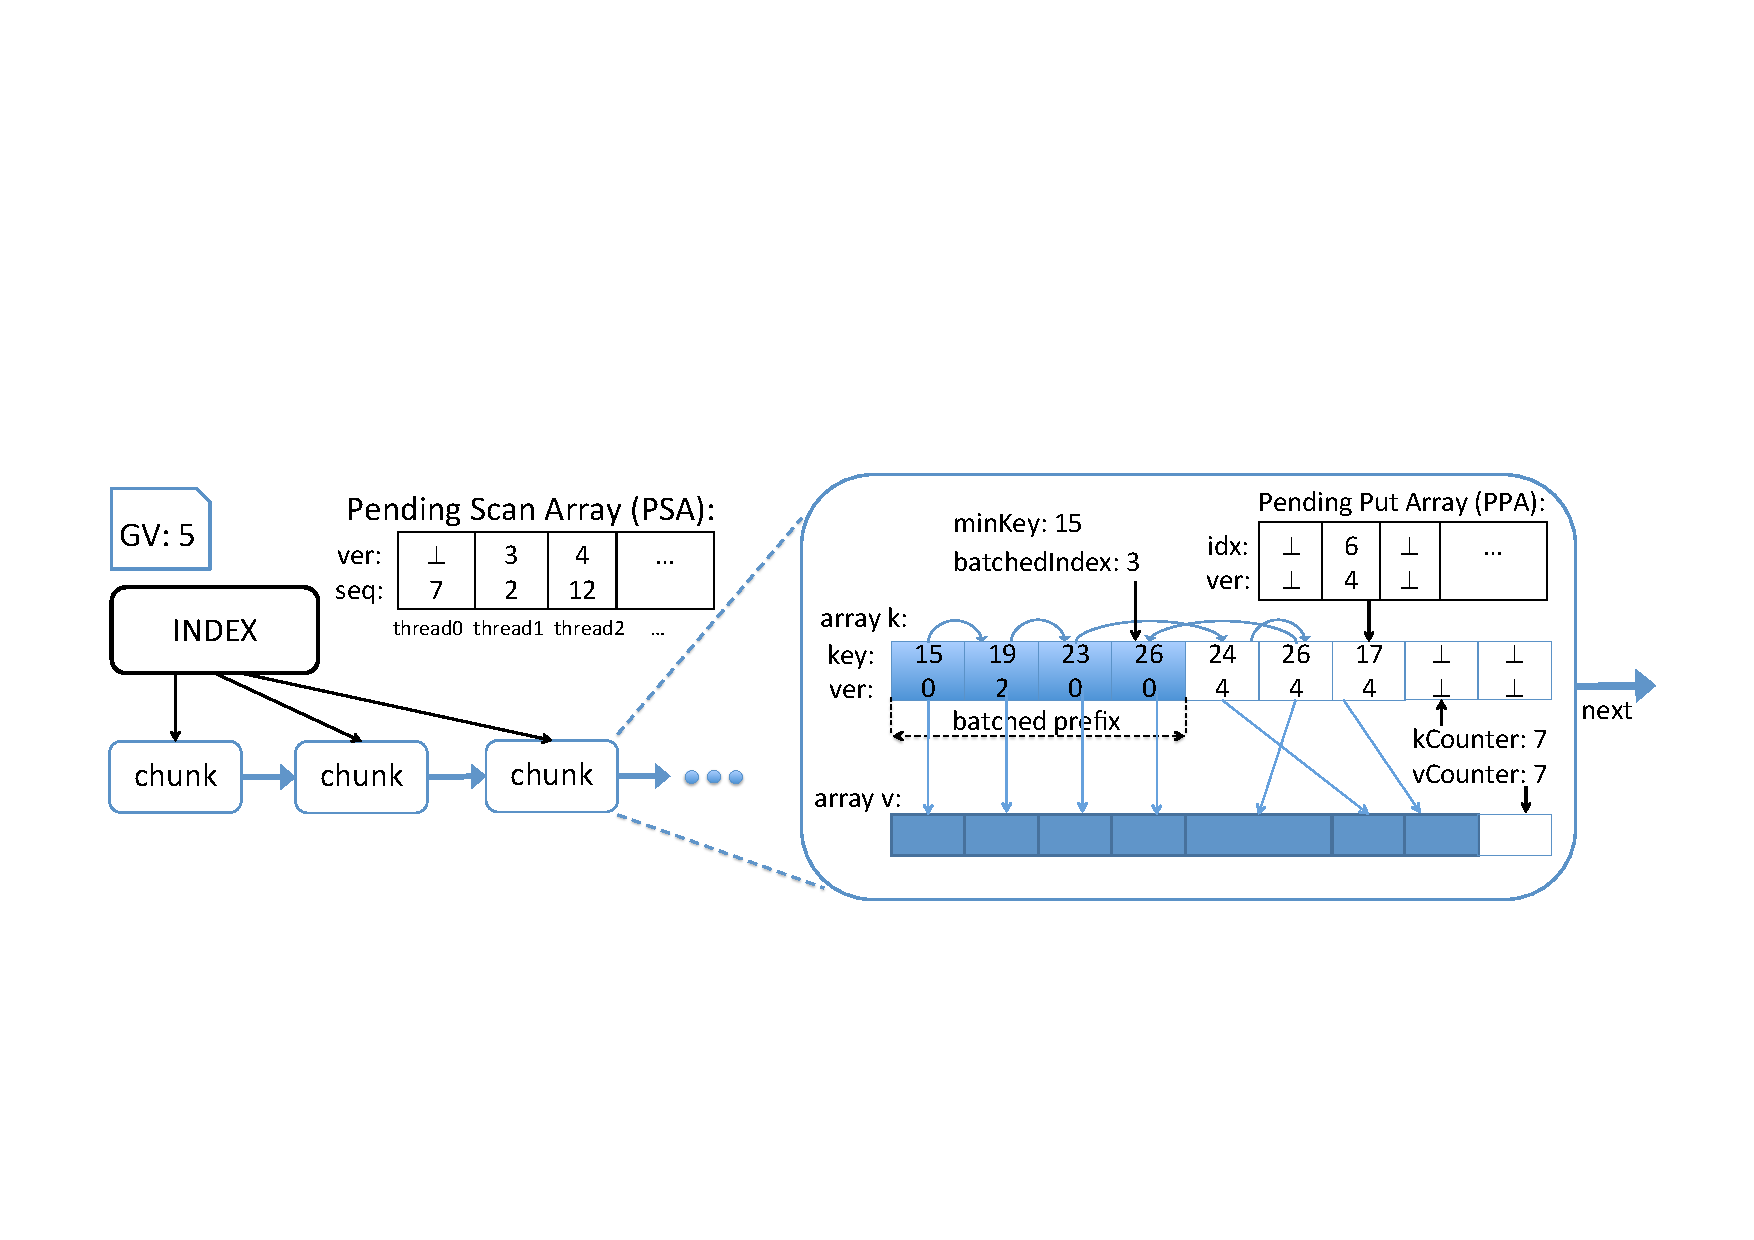
\includegraphics[width=.8\linewidth]{kiwi-layout4.pdf}
  \caption{{{\kiwi} data structure layout. In the zoomed in chunk (on the right), a pending put by the second
thread is attempting to add \code{k[6]} to the linked list with key $17$ and version $4$.}}
  \label{fig:overview-new}
\end{figure*}

\begin{algorithm}[t]
\codesize
\begin{center}
\begin{algorithmic}
%	\State \code{status}	\Comment{infant, normal, or frozen}
	\State immutable \codeF{minKey}  \Comment{minimal key in chunk}
	\State array \codeF{k} of $\langle$key, ver, valPtr, next$\rangle$    \Comment{in-chunk linked list}
	\State array \codeF{v} of values									\Comment{values stored in the list}
	\State \codeF{kCounter, vCounter} \Comment{end of allocated (full) prefixes} % in k and v
	\State \codeF{batchedIndex} \Comment{end of batched prefix in k}
\LineComment pending put array allowing scans and gets to help puts
	\State array \codeF{ppa[{\scshape num\_threads}]} of $\langle$ver, idx$\rangle$
	\State \codeF{next} \Comment{pointer to next chunk in chunk list}
	\State rebalance data $\langle$status, parent, ro$\rangle$ \Comment{rebalancing-related data}
\vspace{-1em}
\end{algorithmic}
\end{center}
\caption{{\kiwi} chunk data structure.}
\label{alg:chunk}
\end{algorithm}


KiWi's chunks are under constant renewal, as the rebalance process removes old chunks and replaces them with new ones.
It not only splits (over-utilized) and merges (under-utilized) chunks as in a B$^{+}$Tree, but also improves their internal
organization, performs \emph{compaction} by eliminating obsolete data, and may involve any number of chunks.
%A \code{status} field in the chunk indicates whether the chunk is undergoing rebalancing, as explained in Section~\ref{sec:rebalance} below.
% an \emph{infant} still being initialized, is a \emph{normal} part of
%the data structure, or is \emph{frozen} for rebalancing purposes.

In order to simplify concurrency control, however, we do not organize chunks in a B$^{+}$tree, but rather in a sorted linked list. This eliminates the synchronization complexity of  multi-level splits and merges.  Yet, to allow fast access, we supplement the linked list with an auxiliary \emph{index} that maps keys to chunks; it may be organized in an arbitrary way (e.g., skip-list or search tree).
Each chunk is indexed according to the minimal key it holds, which is invariant throughout its lifespan. 
(The minimal key of the first chunk in the list is $-\infty$.)
The index supports a wait-free
lookup method that returns the indexed chunk mapped to  the highest key that does not exceed a given {key}. It further supports conditional updates, which are explained in Section~\ref{sec:rebalance}, as they are done only as part of the rebalance procedure. Such updates are lazy, and so
the index may be inaccurate. Therefore, the index-based search is supplemented by a traversal of the chunk linked list.



% Chunk arrays
\paragraph{Intra-chunk organization.}
Each chunk is organized as an array-based linked list, sorted in increasing key order.
KiWi chunks hold two arrays -- \code{v} with written values, and \code{k} with the linked list.
Each cell in \code{k} holds a key, a pointer \code{valPtr}
to a value in \code{v}, and the index of the cell in \code{k} that holds the next key in the linked list.
It also has a version number, as we explain shortly.
When a chunk is created (as a result of rebalancing), some prefix (typically one half) of each array contains data,
and the suffix consists of empty entries for future allocation.

% Batched prefix for efficient binary search
The chunk's full prefix is initialized as sorted, that is, the linked-list successor of each cell is the ensuing cell in \code{k}.
The sorted prefix is called the chunk's \emph{batched prefix}, and it can be searched efficiently using binary search.
As keys are added, the order in the remainder of the chunk is not preserved,
i.e., the batched prefix usually does not grow.
For example, when a key is inserted to the first free cell, it creates a \emph{bypass} in the sorted linked list, where some cell $i$ in the batched prefix
points to the new cell, and the new cell points to cell $i+1$.
We note that in case the insertion order is random, inserted cells are most likely to be distributed evenly in between the batched prefix cells, thus
creating fairly short bypasses.
Given that the prefix and the remainder are of similar sizes, the expected search time remains poly-logarithmic.
Nevertheless, in the worst-case, the search time is linear in the size of the remainder of the chunk.

In order to support atomic scans, KiWi employs \emph{multi-versioning}, i.e., sometimes keeps the old version of a key instead of overwriting it. To this end, KiWi maintains a \emph{global version}, \code{GV}, and tags each key-value pair with a version, \code{ver}. Versions of a key are chained in the linked-list in descending version order. The compaction process that occurs as part of rebalancing eliminates obsolete versions.
Unlike traditional multi-versioning, KiWi creates new versions \emph{only} as needed for ongoing scans.
%This reduces the storage overhead between compactions.
%More importantly,
This allows us to shift the overhead for version management  from updates, which are short and frequent, to scans, which are typically long and therefore much less frequent. Specifically, put operations continue to use the same version (overwriting previous values for written keys, if they exist) as long as no scan operation increases  \code{GV}.


\paragraph{Coordination data structures.}
KiWi employs two %bookkeeping 
data structures for coordinating different operations. 
A global \emph{pending scan array} (PSA) tracks versions used by pending scans for compaction purposes;
each entry consists of a version \code{ver} and a sequence number \code{seq}, as well as the scan's key range.
% in order to avoid ABA races.
A per-chunk \emph{pending put array} (PPA) maps each thread either to a cell in the chunk that the thread is currently attempting to put into and a corresponding version, or $\langle \bot,\bot\rangle$, indicating that the thread is currently not performing a put.
The purpose of the PPA will become evident below.

\subsection{KiWi operations}
\label{sec:ops}

Our algorithm makes use of atomic \emph{compare-and-swap} -- CAS(x,old,new),  \emph{fetch-and-increment} -- F\&I(x), and
\emph{fetch-and-add} -- F\&A(x,a) instructions for synchronizing access to shared data; all impose memory fences.
A pseudocode of \kiwi\ operations is given in Algorithm~\ref{alg:ops}.

\paragraph{Helping puts.}

The interaction between put and scan operations is somewhat involved. In a nutshell, a put uses the current value of \code{GV}, whereas a scan begins by atomically fetching-and-incrementing \code{GV}, causing all future puts to write larger versions than the fetched one. Scan then uses the fetched version, \code{ver}, as its scan time, i.e., it returns for each scanned key the latest version that does not exceed \code{ver}.

However,  a race may arise if
 \code{put(key,val)}  reads a global version equal to \code{ver} for its data and then stalls while a concurrent scan obtains \code{ver} as its scan time and continues to read \code{key} before the put writes \code{val} for \code{key} with  \code{ver}. In this example, \code{val} should be included in the scan (since its version equals the scan time), but it is not (because it occurs late).

We overcome this scenario by having scans \emph{help} pending puts assign versions to values they write. To this end, puts publish their existence in the PPA of the chunk where they write, whereas scans call \code{helpPendingPuts} in each chunk where they read, which 
checks the PPA  and helps any relevant pending put threads it encounters (lines~\ref{l:help-pending}--\ref{l:help-pending-end}).
The helping here is minimal -- it consists of a single CAS that assigns a version to the pending put (line~\ref{l:help-pending-end}).
For example, in Figure~\ref{fig:linearization}, the scan helps \code{put(k1,a)} by setting its version to the current global version, namely $8$.
This orders the put after the scan, so the scan may return the old value.


Since scans use version numbers in order to decide which puts they take into account, the  order of put operations is determined by the order of their versions.
%rather than by the time at which the written value is added to the linked list.
For consistency, gets also need to rely on version numbers.
When a \code{get(key)}  encounters a pending \code{put(key,v)}  with no version, it cannot simply ignore the written value, because the put might end up ordered earlier than the get.
Gets therefore call   \code{helpPendingPuts}  to help pending puts as scans do.
This is depicted in Figure~\ref{fig:linearization}, where the get must help \code{put(k2,b)} obtain a version, because ignoring it
would order the gets inconsistently with the version order that would later be
observed by the scan.
%\todo{Add cross-reference to proof.}


\begin{figure}[tb]
\centerline{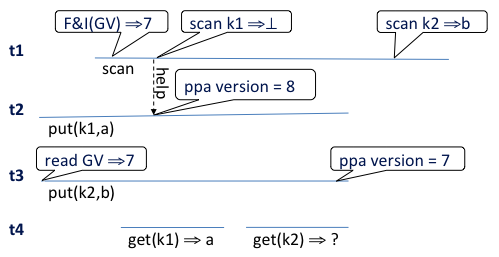
\includegraphics[width=0.85\columnwidth]{kiwi-linearization.png}}
\caption{Example of scan operation enforcing order between puts:
%according to version numbers:
The \code{scan} assigns
\code{put(k1,a)} a new version ($8$), whereas \code{put(k2,b)} later completes with an old version ($7$).
We see that if \code{get(k2)} does not help \code{put(k2,b)}, the gets see puts in a  different order than the  scan.
}
\label{fig:linearization}
\end{figure}

\paragraph{Put implementation.}


\begin{algorithm*}[tb]
\codesize
         \begin{multicols}{2}
	\begin{algorithmic}[1]{}

		\Procedure{put}{key, val}	
 \LineComment {\em 1. prepare cell to insert}
		\State locate target chunk $C$
\label{l:put-prep}
		\If{\codeF{checkRebalance($C$, \codeF{key, val}})}   \label{l:put-rebalance0}
			\State return \Comment{required rebalance completed the put}
		\EndIf
		\State \codeF{j} $\leftarrow$ F\&A($C$.\codeF{vCounter, val.size}) \Comment{allocate place for value}
		\State \codeF{i} $\leftarrow$ F\&I($C$.\codeF{kCounter}) \Comment{allocate cell in linked list}
		\If{ \codeF{j} $\geq$ \codeF{$C$.v.size} $\vee$  \codeF{i} $\geq$ \codeF{$C$.k.size}} 
			\If {$\neg$\codeF{rebalance($C$,\codeF{key, val})}} \codeF{put(key, val)}  \EndIf 
		\EndIf
		\State \codeF{v[j]} $\leftarrow$ \codeF{val}
		\State \codeF{k[i]} $\leftarrow \langle\codeF{key}, \bot, \codeF{j}, \bot\rangle$ \Comment{version and list connection not set yet}
\label{l:put-prep-end}
 \LineComment {\em 2. get version via PPA}
		\State \codeF{$C.$ppa[t].idx}  $\leftarrow$  \codeF{i}
\label{l:put-version}
		\State \codeF{gv} $\leftarrow$ \codeF{GV}      \label{l:put-LP}
		\State CAS($C.$\codeF{ppa[t]}, $\langle \bot$, \codeF{i} $\rangle$, $\langle$ \codeF{gv, i} $\rangle$) \label{l:put-cas-version}
		\If{\codeF{$C.$ppa[t].ver = frozen}} %%% or $C$.\codeF{status = frozen}}
		\Comment{$C$ is being rebalanced \label{l:put-frozen}}
			\If {$\neg$\codeF{rebalance($C$,\codeF{key, val})}} \codeF{put(key, val)}  \EndIf    		\label{l:put-restart}
		\EndIf
		\State  $C$.\codeF{k[i].ver}  $\leftarrow$   \codeF{$C.$ppa[t].ver}
\label{l:put-version-end}
 \LineComment {\em 3. add \codeF{k[i]} to linked list}
	\Repeat		
\label{l:put-ll}
		\State \codeF{c}$ \leftarrow$ \codeF{find(key, k[i].ver, $C$)} \Comment{search linked list $C.$\codeF{k}}
		\State						\Comment{use binary search up to $C.$\codeF{batchedIndex}}
		\If{\codeF{c} $= \bot$} \Comment{not found}
			\State link $C$.\codeF{k[i]} to the list using CAS \label{l:put-insert1}
			\If{CAS succeeded} break \EndIf
		\ElsIf{\codeF{c.valPtr} =  \codeF{j'}$<$\codeF{j}} \Comment{overwrite}
				\State  CAS(\codeF{c.valPtr, j', j}) \label{l:put-insert2}
		\EndIf		
	\Until{\codeF{c.valPtr} $ \geq$ \codeF{j}}
\label{l:put-ll-end}
%	\LineComment clean up
	\State  \codeF{ppa[t]} $\leftarrow \langle \bot, \bot \rangle$
\label{l:put-clean}
	\EndProcedure

\Statex
\Statex

	\Procedure{get}{key}	
		\State locate target chunk $C$ \label{l:get-start}
		\State \codeF{helpPendingPuts($C$, key, key)}
		\State return \codeF{findLatest(key, $\infty$, $C$)}
	\EndProcedure

\Statex

		\Procedure{scan}{fromKey, toKey}	
	 \LineComment {\em 1. obtain version - synchronize with rebalance via PSA}
		\State \codeF{psa[t]}  $\leftarrow$ $\langle ?$,\codeF{seq, fromKey, toKey}$\rangle$ \Comment{\codeF{seq} is a thread-local counter    \label{l:scan-version}}
		\State \codeF{ver} $ \leftarrow$ F\&I(GV)
		\State CAS(\codeF{psa[t]}, $\langle ?$,\codeF{seq, fromKey, toKey}$\rangle$, $\langle$\codeF{ver,seq, fromKey, toKey}$\rangle$)
			 \label{l:scan-FiCAS}
		\State \codeF{ver}  $ \leftarrow$  \codeF{psa[t].ver}
%%%  \Comment{accounts for the case that a version had already been assigned}
\label{l:scan-version-end}
	 \LineComment {\em 2. scan relevant keys}
		\ForAll{chunk $C$ in query range} \label{l:scan-scan}
			\State \codeF{helpPendingPuts($C$, fromKey, toKey)}
			\ForAll{key in query range}
				\State return \codeF{findLatest(key, ver, $C$)}
			\EndFor
		\EndFor \label{l:scan-scan-end}
%		\State \codeF{seq++} \label{l:scan-version}
		\State \codeF{psa[t]}  $\leftarrow$ $\langle\bot$,\codeF{seq++}$\bot, bot, \rangle$
	\EndProcedure

%\Statex
\Statex

	\Procedure{helpPendingPuts}{fromKey, toKey, $C$}  \label{l:help-pending}
			\ForAll {entry $e$ in $C$.\codeF{ppa}} 				
				\State \codeF{idx} $\leftarrow$ $e$.\codeF{idx} 
				\If{ $C$.\codeF{k[idx].key} $\in$ [\codeF{fromKey, toKey}]} 
					\State \codeF{gv} $\leftarrow$ \codeF{GV}  \label{l:get-readGV}
					\State CAS($e$, $\langle \bot$, \codeF{idx} $\rangle$, $\langle$ \codeF{gv, idx} $\rangle$)  \label{l:get-help}
					\label{l:help-pending-end}
				\EndIf
			\EndFor		
	\EndProcedure	

\Statex

	\Procedure{findLatest}{key, ver, C}  \label{l:find-latest}
%		\LineComment find cell in $C$ with \codeF{key} and highest version up to \codeF{ver} %, breaking ties using \codeF{valPtr}
		\State search \codeF{key} in $C$.\codeF{k} and \codeF{ppa}
% using binary search up to $C.$\codeF{batchedIndex} and then linear traversal	
%		\State search \codeF{key} in \codeF{ppa}
%		\If{found at least one cell with \codeF{key} and \codeF{ver}}
%			\State return  one with  highest \codeF{valPtr}
%		\EndIf
		\If{found at least one cell with \codeF{key} and version $\leq$\codeF{ver}}
			\State return one with highest version, break ties by \codeF{valPtr}
		\EndIf
	\State return $\bot$
	\EndProcedure	

	\algstore{kiwi} %% Uncomment to add another pseudocode figure
	\end{algorithmic}
	\end{multicols}
	\caption{\kiwi\ operations -- pseudocode for thread \code{t}.}
	\label{alg:ops}
\end{algorithm*}


The put operation appears in the left column of Algorithm~\ref{alg:ops}. It
consists of three phases: (1) locate the target chunk and
prepare a cell to insert with the written value; (2) obtain a version while syncrhonizing with
concurrent scans, gets, and rebalances via the PPA; and (3) connect  the new cell to the linked list.

%For simplicity we describe the algorithm as if both the key and value are embedded in the cell; in practice, to support variable length values the cell %can consist of pointer to where the value is stored.

The first phase (lines~\ref{l:put-prep}--\ref{l:put-prep-end})
locates the target chunk $C$, traversing the index and the linked list if needed. Later this phase allocates space for the key and the variable-length value, by increasing $C$'s array  counters to the next available indices \code{i} and \code{j} for \code{k} and \code{v}, resp.
This is done using atomic F\&I and F\&A, so in case of concurrent put operations, each thread gets its own cells.

Before increasing \code{i} and \code{j}, put checks if rebalancing is needed, because the chunk is full, imbalanced, or immutable, 
as discussed in the next section. This is done by the procedure \code{checkRebalance} given below, 
which returns \code{false} in case no rebalance is needed, and otherwise completes (or restarts) the put.
%, which restarts the put operation in case it needs to rebalance.  
After increasing \code{i} and \code{j}, put verifies that they are not too large, 
and if so, proceeds to write values into \code{k[i]} and \code{v[j]}, without a version at this point; note that \code{k[i]} is not yet connected to the linked list.

The second phase (lines~\ref{l:put-version}--\ref{l:put-version-end}) publishes \code{i} in the thread's entry in $C$'s PPA,
and then uses CAS to set the version to the current value of \code{GV}.
The CAS may fail in two possible ways. First, if the chunk is undergoing rebalancing, then
the reblanacing thread may have set the thread's PPA version to \code{frozen}.
In this case, the put cannot proceed since the chunk is deemed immutable. Instead, it invokes \code{rebalance}, 
and if rebalance returns false indicating that it did not insert the put's key and value, the put restarts
(lines \ref{l:put-frozen}--\ref{l:put-restart}).
(Invoking rebalance on a chunk that is already being rebalanced is done for lock-freedom, given that the original rebalancing thread
may be stalled.)
Second, a helping thread may have already set the version;
to account both for this case and for the case CAS succeeds,
put uses the version from the PPA, and copies it to \code{k[i]} (line \ref{l:put-version-end}).

The third phase, (lines~\ref{l:put-ll}--\ref{l:put-ll-end}), adds \code{k[i]} to the linked list.
To find the insertion point, it first uses binary search on the batched prefix and then traverses the remaining linked list.
If the linked list does not contain a cell with the same key and version, then \code{k[i]} is linked to the list (line \ref{l:put-insert1}).
Otherwise, ties between two puts with the same key and version are broken based on the indices of their allocated cells in \code{v}.
If the put that allocates cell \code{j} finds in the linked list a cell with index \code{j'} with the same key and version such that \code{j'}$<$\code{j},
it uses CAS to replace that cell's \code{valPtr} to point to \code{v[j]} (line \ref{l:put-insert2}).
If \code{j'}$>$\code{j} then the put does nothing, since its value has effectively been overwritten.
Note that in both cases some cell, either \code{j} or \code{j'}, remains allocated but is not connected to the linked list.
%Namely, at most one cell with a given key-version pair is connected to the linked list.
Unconnected cells are compacted by the  rebalancing process.
Finally, the PPA version is cleared (line \ref{l:put-clean}).
%using a CAS (line \ref{l:put-clean}).
%The CAS is used to account for a race with a concurrent rebalancing thread that attempts to set the version to \code{frozen}.

\paragraph{Gets and scans.}

Gets and scans are presented in the right-hand column in Algorithm~\ref{alg:ops}.
A \code{get(key)} begins by querying the index for \code{key}, and then (if needed), traverses the linked-list of chunks until
the next chunk's \code{minKey} exceeds \code{key} (line \ref{l:get-start}).
If there is a pending put to \code{key} that does not have a version yet, (i.e., its version is $\bot$), get attempts to help it by setting its version to
the current value of \code{GV} using CAS  (line \ref{l:get-help}). (CAS may fail in case the put sets its own version or is helped or frozen by another thread).
It then calls \code{findLatest()}  to find the latest version of the searched key.

The \code{findLatest()} function (line~\ref{l:find-latest}) performs a binary search on the batched prefix, and continues to traverse the in-chunk linked list until it either finds  \code{key} or finds that it does not exist. In addition, \code{findLatest()} checks the PPA for potential pending puts of the target key,
ignoring entries with no versions as these were added after the help.
In case multiple versions of \code{key} exist, it returns the one with the highest version.
If a pending put has the same version for the sought key as an entry in the linked list, then the one with the larger \code{valPtr} is returned.

A scan first determines its scan time  (lines \ref{l:scan-version}--\ref{l:scan-version-end}).  It obtains a  unique version via F\&I of \code{GV},
and attempts to set it as its scan time while synchronizing itself relative to helping rebalance operations
as described below.

It then reads all the keys in the relevant range (lines \ref{l:scan-scan}--\ref{l:scan-scan-end})
by traversing the list of chunks, and within each chunk, proceeding as get does to help all pending puts and find the latest version of each key.

\paragraph{Ordering operations.}



\begin{table}[t]
\codesize
\begin{center}
\begin{tabular}{|l|c|c|c|}

 \hline
 {\bfseries } 		& {\bfseries scan}			& {\bfseries put }    	& {\bfseries rebalance }	\\
 \hline

 {\bfseries scan}       & F\&I 	\codeF{GV}  	& \textendash				& \textendash			\\
% 				& \codeF{GV}     		& 						& 					\\
\hline
 {\bfseries put } 	& CAS		 		& by version, then	 		& \textendash			\\
 			        &  \codeF{ppa[t].ver} 		& F\&A \codeF{vCounter} 		& 				\\
\hline
 {\bfseries rebalance}& 	CAS				& CAS  to \codeF{frozen}   		& CAS \\
				& 	\codeF{psa[t].ver} 			& \codeF{ppa[t].ver}   		& \codeF{rebalanceObj} \\
 \hline

\end{tabular}
\end{center}
\caption{Atomic operations and rendevouz points determining order between \kiwi\ procedures.}
\label{tab:sync}
\end {table}

The  order among concurrently executing \kiwi\ procedures is determined by atomic hardware operations
(F\&I, F\&A, or CAS) on pertinent memory locations.
Table~\ref{tab:sync} summarizes the rendevouz points for different types of operations. For brevity, we omit gets from the table.

Each scan has a unique version. The order between concurrent scans is determined by
the order in which they (or the rebalance threads that help them) perform F\&I on \code{GV}.
Scans (and gets) order themselves relative to a put by thread \code{t} via \code{ppa[t].ver} in the chunk where the put occurs.

The order between puts that attempt to  insert the same key is determined by their versions, which reflects their order wrt ongoing scans.
Puts that have the same version, (i.e., the order between them is not determined by scans), are ordered according to
the order in which they succeed to fetch-and-add  \code{vCounter}.
Rebalance operations are discussed below.




\subsection{Rebalancing}
\label{sec:rebalance}

Section~\ref{sec:rebalance-trigger} discusses the life-cycle of a \kiwi\ chunk, and in particular,
when it is rebalanced. Section~\ref{sec:rebalance-stages} then walks through the stages of the rebalance process.

\subsubsection{Triggering rebalance and chunk life-cycle}
\label{sec:rebalance-trigger}

We saw that put calls \code{checkRebalance($C$)} in line~\ref{l:put-rebalance0} of Algorithm~\ref{alg:ops} before adding a new key to $C$.
This procedure triggers \code{rebalance($C$)} whenever $C$ is full or otherwise unbalanced, according
to some specified \emph{rebalance policy}; we refer to $C$ as the \emph{trigger chunk} of the rebalance.

To address the immediate problem, \kiwi\ could, in principle, restrict itself to the trigger chunk:
It can free up space by \emph{compacting} $C$, i.e., removing deleted values, values that are no longer in the linked list
because their keys have been over-written, as well as values that pertain to old versions that are not required by any active scan;
if this does not suffice (because all the information in $C$ is needed), \kiwi\ may \emph{split} the chunk.
Furthermore, it can address the imbalance  by \emph{sorting} the chunk.

The problem with this approach is that it may leave under-utilized chunks in the data structure forever.
\kiwi\ improves space utilization by allowing chunks to \emph{merge}, or more generally,
\emph{engaging} a number of old chunks in the rebalance,
and replacing all of them with any number of new ones.
The chunks to engage are determined by the rebalance policy.

Rebalance clones the relevant data from all engaged chunks  into new chunks, and then
replaces the engaged chunks with the new ones in the data structure.
Cloning creates a window when the same data resides at two chunks -- new and old.
In order for get and scan to be wait-free, the chunks remain accessible for reading during this period.
But in order to avoid inconsistencies, both chunks (old and new) are immutable throughout the window.

This defines a life cycle for chunks: they are created as immutable \emph{infants} by some \emph{parent} trigger chunk $C$;
they become \emph{normal} mutable chunks at the end of the rebalance process; and finally, they become \emph{frozen}
(and again immutable) when they are about to be replaced.
(We assume that a complementary garbage-collection mechanism eventually removes disconnected, frozen chunks.)
%after there are no pointers to them.
%from the chunk linked list, the index, or active threads.
The chunk's status (infant, normal, or frozen), the pointer to parent, and the pointer to rebalance object are part of the rebalance data
stored in the chunk (see Algorithm~\ref{alg:chunk}).


The \code{checkRebalance($C$)} procedure is given in Algorithm~\ref{alg:rebalance}. 
It checks whether $C$ is immutable, and if so, helps complete the process that makes it immutable
($C$'s parent in case $C$ is an infant, and $C$ in case it is frozen).
The rebalance procedure consists of two functions, \codeF{rebalance} and \codeF{normalize}; in case
the chunk's parent is helped only the latter is perfromed as explained below.
In addition, if the chunk is full or if the rebalance policy chooses to do so, it also triggers rebalance on $C$.
Note that put calls \code{checkRebalance} before incrementing \code{kCounter} and \code{vCounter} in order to avoid filling up infant chunks.
The \code{reblance} procedure takes the put's key and value as parameters, and attempts to piggyback the put on the reblanace, i.e., insert the key and value to the newly created chunk. In case it fails, it returns false, in which case the put is restarted. 

\begin{algorithm}[tb]
\codesize
	\begin{algorithmic}[1]{}
		\algrestore{kiwi} %% Uncomment to add another pseudocode figure
		\Procedure{checkRebalance}{$C$, key, val}
		\If{\codeF{$C$.status=infant}} 
			\State normalize($C$.parent)
			\State \codeF{put(key, val)} 
		\EndIf
		\If{\codeF{$C$.vCounter} $\geq$ \codeF{$C$.v.size} $\vee$ \codeF{$C$.kCounter} $\geq$ \codeF{$C$.k.size} $\vee$ 
			\State \codeF{$C$.status = frozen}  $ֿֿ\vee$ \codeF{policy($C$)} 
			} 
			\State ok $\leftarrow$ \codeF{rebalance($C$, key, val)}
			\State normalize($C$)
			\If {$\neg$ok} \codeF{put(key, val)} \EndIf 
		\EndIf
		\EndProcedure
		\algstore{kiwi} %% Uncomment to add another pseudocode figure
	\end{algorithmic}
\caption{The checkRebalance procedure.}
\label{alg:check-rebalance}
\end{algorithm}	


The  policy will typically choose to rebalance $C$ whenever $C$ is full or under-utilized, as well as when
its  batched prefix becomes too small relative to the number of keys in $C$'s linked list.
In order to stagger rebalance attempts in case of many insertions to the same chunk,
the policy can make probabilistic decisions:  If a chunk  is nearly full or somewhat under-utilized or
unbalanced, then the policy may flip a coin to decide whether to invoke rebalance or not.
%Of course, if the chunk already full, it needs to be rebalanced immediately.

\subsubsection{Rebalance stages}
\label{sec:rebalance-stages}

\newenvironment{compactenum}
{ \begin{enumerate}
    \setlength{\itemsep}{0pt}
    \setlength{\parskip}{0pt}
    \setlength{\parsep}{2pt}     }
{ \end{enumerate}      }

Rebalance  proceeds in the following seven stages:
\begin{compactenum}
\item \emph{Engage} -- agree on the list of chunks to engage.
\item \emph{Freeze}  -- make engaged chunks immutable.
\item \emph{Pick minimal version} --  to keep in compaction.
%, after helping pending scans obtain versions.
\item \emph{Build} -- create infant chunks to replace engaged ones.
\item \emph{Replace} -- swap new chunks for old ones in  list.
\item \emph{Update index} -- unindex old chunks,  index new ones.
\item \emph{Normalize} -- make the new chunks \emph{mutable}.
\end{compactenum}

If the first check of \code{checkRebalance()} decides to help rebalance a chunk's parent, then
rebalance starts in stage $6$, since the chunk's reachability implies that stage $5$ is complete.
In the other two cases, (a frozen chunk or a new trigger chunk), rebalance cycles through all seven stages.
This is safe because all stages are idempotent, and ensures lock-freedom, namely, progress in case the original rebalance stalls.
The first five stages are performend in the \codeF{rebalance} procedure, whereas the last two are performed in \codeF{normalize}.
\inote{A pseudo-code for the rebalance process is given in Algorithm~\ref{alg:check-rebalance}.
We now describe the stages in detail.}
%
For space limitations we omit the rebalance pseudocode; we now describe the seven stages.

\begin{algorithm*}[th]
\codesize
         \begin{multicols}{2}
	\begin{algorithmic}[1]{}
	\algrestore{kiwi}
	\Procedure{rebalance}{$C$, put\_key, put\_val}	
	\LineComment {\em 1. engage }
	\State \codeF{ro} $\leftarrow$ new rebalance object, initially $\langle C, C.\codeF{next}, \bot \rangle$
	\State \codeF{last} $\leftarrow C$
	\State CAS($C$.\codeF{ro}, $\bot$, \codeF{ro})
	\State \codeF{ro} $\leftarrow$ $C$.\codeF{ro}
	\While{ \codeF{ro.next} $\not=\bot$ }
		\State \codeF{next} $\leftarrow$ \codeF{ro.next}
		\If{\codeF{policy(next)}} \Comment{try to engage next}
		 	\State CAS(\codeF{next.ro}, $\bot$, \codeF{ro}) 
		 	\If{\codeF{next.ro = ro}}  \Comment{engaged next}
		 		\State CAS(\codeF{ro.next}, \codeF{next}, \codeF{next.next}) 
		 		\State \codeF{last} $\leftarrow$  \codeF{next}
			\Else 		 		
				\State  CAS(\codeF{ro.next}, \codeF{next}, $\bot$) 	
			\EndIf
		\Else 		 		
			\State  CAS(\codeF{ro.next}, \codeF{next}, $\bot$) 	
		\EndIf
	\EndWhile

	\LongLineComment {search the last concurrently engaged chunk}
	\ForAll{chunks \codeF{c} from \codeF{last} s.t. \codeF{c.ro} $=$ \codeF{ro}}
		\State \codeF{last} $\leftarrow$ \codeF{c}
	\EndFor

	\LineComment {\em 2. freeze}
	\State $C$.\codeF{status} $\leftarrow$ \codeF{frozen}
			\ForAll {entry $e$ in $C$.\codeF{ppa}} 				
				\State \codeF{idx} $\leftarrow e$.\codeF{idx} 
				\State CAS($e$, $\langle\bot$, \codeF{idx}$\rangle, \langle$\codeF{frozen, idx}$\rangle$)  
			\EndFor		

	\LineComment {\em 3. pick minimal version}

	\ForAll{\codeF{psa[t] = $\langle$?, seq, from, to$\rangle$}}
		\If{$C$.minKey $\le$ to $\wedge$ 
			\State $C$.next.minKey $>$ from} 
			\State add { $\langle$t, seq, from, to$\rangle$} to \codeF{toHelp}
		\EndIf
	\EndFor				
	\If{toHelp $\not=\emptyset$}
		\State \codeF{ver} $ \leftarrow$ F\&I(GV)
		\ForAll{$\langle$t, seq, from, to$\rangle \in$  \codeF{toHelp}}  
				\State CAS(\codeF{psa[t]}, $\langle$?,\codeF{seq,from,to}$\rangle, \langle$\codeF{ver,seq,from,to}$\rangle$)
		\EndFor
	\EndIf

	\vspace{10mm}
	\LineComment {\em 4. build}
	\LongLineComment{we assume the \# of versions is much smaller than the chunk size}
	\State $C_f \leftarrow C_n \leftarrow$ new chunk  
		\State \hspace{5mm} with \codeF{minKey}=$C$.\codeF{minKey}, \codeF{parent}=$C$, \codeF{status=infant} 
	\ForAll{chunks $C_o$ from \codeF{ro.first} to \codeF{last}}
		\If{$C_o$.\codeF{minKey} $<$ \codeF{put\_key} $<$ $C_o$.\codeF{next.minKey}}   
			\State  \codeF{toPut} $\leftarrow \{ \langle$\codeF{put\_key},GV, \codeF{put\_val}$\rangle \}$
		\Else
			\State \codeF{toPut} $\leftarrow \emptyset$
		\EndIf
		\ForAll{keys k in $C_o \cup $\codeF{toPut} in sorted order}
			\If{$C_n$ is more than half full} 
				\State $C_n$.\codeF{next} $\leftarrow$  new chunk 
					\State \hspace{5mm} with 
					\codeF{minKey}=$C$.\codeF{k}, \codeF{parent}=$C$, \codeF{status=infant} 
				\State $C_n \leftarrow C_n.$\codeF{next}
			\EndIf
			\ForAll{versions $\langle$ ver, val $\rangle$ of k, in descending order}
				\State insert $\langle$ k, ver, val $\rangle$ to $C_n$
				\If{ver $<$ \codeF{minKey}} break \EndIf
			\EndFor
		\EndFor
	\EndFor
	\LineComment {\em 5. replace}
	\State \codeF{last.immutable} $\leftarrow$ true
	\State $C_n$.\codeF{next} $\leftarrow$ \codeF{last.next}
	\State \codeF{pred} $\leftarrow$ $C$'s predecessor
	\If{CAS(\codeF{pred.next+immutable}, $C$+false, $C_f$+false)} 
		\State return true  \Comment{insertion succeeded}   \EndIf
	\If{\codeF{pred.next.parent} = $C$} 
		\State return false \Comment{someone else's insertion succeeded}
	\Else \Comment{insertion failed, help predecessor and retry}
		\State rebalance(pred, $\bot, \bot$)
		\State return rebalance($C$, put\_key, put\_val)
	\EndIf 

	\EndProcedure
	
	\Statex
	
	\Procedure{normalize}{$C$}	
	\LineComment {\em 6. update index}
	\ForAll{chunks $c$ from $C_f$ to $C_n$}
		\State load: \codeF{index.loadPrev($c$.minKey)}
		\If {$\neg c$.\codeF{frozen}}
			\If{$\neg$ \codeF{index.putConditional($c$.minKey, $c$)}}
				goto load 
			\EndIf 
		\EndIf
	\EndFor		
	\ForAll{chunks $c$ from \codeF{ro.first} to \codeF{last}}
			\State \codeF{index.deleteConditional($c$.minKey, $c$)}
	\EndFor
	\LineComment {\em 7. normalize}	
	\ForAll{chunks $c$ from $C_f$ to $C_n$}
		$c$.\codeF{status $\leftarrow$ normal}
	\EndFor		
	\EndProcedure

		\end{algorithmic}
	\end{multicols}
\caption{\kiwi's rebalance operation.}
\label{alg:rebalance}
\end{algorithm*}	

\paragraph{1. Engagement.}



Since multiple threads may simultaneously execute \code{rebalance($C$)}, they need to reach \emph{consensus} regarding
the set of engaged chunks. The consensus is managed via pointers from the chunks to a dedicated rebalance object \code{ro}.
Once a chunk is engaged in a rebalance it cannot be engaged with another rebalance.
The engaged chunks in a particular rebalance always form a contiguous sector of the chunks linked list.
For simplicity, this sector always starts from the trigger chunk forward,  though in principle it is possible
to grow the sector backwards from the trigger chunk as well.
A rebalance object holds pointers to three chunks, \code{first} (the trigger chunk) and \code{next} 
(the next potential chunk to engage in the rebalance).
%A rebalance object holds pointers to three chunks, \code{first}, \code{next} and \code{last}, where \code{first} is
%the trigger chunk,  \code{next} is the next potential chunk to engage in the rebalance,
%and \code{last} is the (agreed-upon) final chunk of the rebalance.
%, after all the nodes between the trigger chunk and it have been engaged.
The engagement  preserves the following invariant:
\begin{invariant}
Consider a rebalance object \code{ro}.
If \code{ro.next}${\not=}{\bot}$ then
for every chunk $C$ in the linked list from \code{ro.first} to the chunk before \code{ro.next}, \code{$C$.ro=ro}.
\end{invariant}


%Algorithm~\ref{alg:engage} includes pseudocode for engagement, which
Engagement
begins by agreeing on the \code{ro} to use. This is done by (1) creating a rebalance object
 referring to the trigger chunk $C$, (2) attempting to set \code{$C$.ro}
to the new rebalance object via CAS, and (3) using the \code{ro} in \code{$C$.ro}.
Note that the latter was set by a successful CAS of some rebalance thread.
Next, we try to engage ensuing chunks in the list one by one.
In each iteration, we consult the policy whether to engage the next chunk.
We then use CAS to change \code{ro.next} to either \code{ro.next.next}, or $\bot$ indicating
that it is time to stop engaging chunks.
We exit the loop when \code{ro.next} is $\bot$, and then set the local variable \code{last} 
to  the last engaged chunk.


\paragraph{2. Freezing.}

Once the list of engaged chunks is finalized, we freeze them so no data will be added to them
while they are being cloned. Recall that puts become visible to concurrent retrievals once they
publish themselves in the chunk's PPA, and that before doing so, they check if the chunk
is frozen. However, we need to account for the scenario where a chunk becomes frozen after
put checks its status and before the put publishes itself in PPA.
To this end,
rebalance traverses all PPA's entries and attempts to set their versions to frozen using CAS.
If the CAS is successful, the put will fail to assign itself a version
(Algorithm~\ref{alg:ops}, line~\ref{l:put-restart}). Otherwise, the put has already assigned its version, and
rebalance can take it into account during cloning.
\inote{
As an optimization, it is possible to help pending puts perform the actual linked-list insertion
in order to avoid the need to clone data from the PPA.
}

\paragraph{3. Determining the minimal read version and helping scans.}

We need to clone all data versions that might still be needed by scans.
To this end, we compute \code{minVersion}, the minimum read point among all active  and future scans --
this is the smallest version among those published in PSA and the current \code{GV}.

Since a scan cannot atomically obtain a scan time from \code{GV} and publish it in PSA,
rebalance cannot ignore scans that have started but did not publish a version yet.
We therefore use a helping mechanism: scan first publishes ? in PSA (Algorithm~\ref{alg:ops}, line~\ref{l:scan-version})
indicating its intent to obtain a version, then fetches-and-increments the global version
and uses CAS to update the version from ? to the one it obtained.

Concurrent rebalance operations help scans install a version in started entries;
monotonically increasing counters are used to prevent ABA races where an old rebalance ``helps'' a new scan.
Specifically, rebalance does the following: (1) it scans the  PSA for entries with ? whose range overlaps the
range covered by the engaged chunks; (2) if any are found, it fetches-and-increments \code{GV} and
reads its new version into \code{gv}; (3) for every \code{psa[t]}=  $\langle$?, $n \rangle$ entry found in (1),
it attempts to CAS \code{psa[t]} to  $\langle$\code{gv}, $n \rangle$.
Note that scan's CAS (line~\ref{l:scan-FiCAS})  might fail  in case it is helped, but
either way, it uses the version written by some successful CAS (line~\ref{l:scan-version-end}).


\paragraph{4. Creating new chunks and completing the put.}

The next stage creates new chunks to replace the engaged ones. It traverses the list of engaged chunks from \code{ro.first} to \code{last}.
In each chunk, it collects data both from the intra-chunk linked list and from the PPA. Additionally, 
the key and val of the put that triggered the rebalance is included in the appropriate chunk. 
All versions of a key that are older than the last version that does not exceed \code{minVersion} can be safely discarded, whereas
newer versions are cloned into new chunks. New chunks are created one at a time, as infants, with the trigger chunk as their parent.
%, and the intra-chunk linked list sorted.

Keys are added, in sorted order, to a new chunk $C$ until it is roughly half full, at which point a new chunk $C'$ is created
and $C.\code{next}$ is set to $C'$. (In case the last chunk is too sparse, for example, only a quarter full, it is discarded and its keys are moved to the  penultimate chunk).

\paragraph{5. Data structure update.}

Next, rebalance attempts to insert the new section into the linked list instead of the engaged one.
This involves two steps: First, the \code{next} pointer of the tail chunk in the new section needs to take the value of
the \code{next} pointer in \code{last}. Second, the \code{next} pointer of the predecessor of \code{ro.first} needs to be set to the head of
the new chunks' list. In order to execute the two steps atomically, we do the following:
(1) \emph{mark} the \code{next} pointer in \code{last} as immutable;
(2) set the tail of the new chunk sector to its value; and
(3) use CAS to set the \code{next} pointer of the predecessor of \code{ro.first}.

If CAS succeeds, we return true.
If CAS fails because another rebalance (using the same rebalance object) has successfully replaced the trigger chunk with a new one, we simply return false (indicating that the new key and value were not added as part of the rebalance, and hence put should restart) 
without taking any additional actions. But if CAS fails because some other rebalance had marked the \code{next} pointer as immutable (step (1) above), then we recursively help that rebalance complete, and then re-attempt to insert the new chunk sector to the list.

In the special case when the new list is empty (because no data is kept), step (3) CASes  the \code{next} pointer of the predecessor of \code{ro.first} to the  \code{next} pointer of \code{last}.

\paragraph{6. Index update.}

%The next phase adds the new chunks to the index and removes  the replaced ones.
Since the new chunks are already accessible via the linked list and the old chunks are already frozen, the index update can be lazy, and updates of different chunks can proceed without synchronization.
Nevertheless, we need to take into account races with old rebalance operations--- a thread that wakes up after being stalled must be prevented from indexing a chunk that had already been supplanted.

To this end, we assume that the index supports a form of semantic load-linked and store-conditional; specifically, it provides the following API:
(1) \code{loadPrev(k)} --- returns the indexed chunk mapped to the highest key that does not exceed \code{k};
(2) \code{deleteConditional(k,$C$)} --- removes key \code{k} only if mapped to chunk $C$; and
(3) \code{putConditional(k,prev,$C$)} --- maps \code{k} to $C$ provided that the highest key in the index that does not exceed
\code{k} is mapped to \code{prev}.
Such an index can be implemented in non-blocking ways using low-level atomic operations \cite{BraginskyP2012}; in our implementation,
we instead use locks.

To index a new chunk $C$, we first call \code{loadPrev($C$.minKey)}, then verify that $C$ is not frozen, and if so,
add it conditionally to the index. If the conditional put fails and yet the chunk is not frozen, the put is retried.
Index removals call \code{deleteConditional(C.minKey,C)}.

\paragraph{7. Normalization.}
Finally, the status of the new chunks is set to normal, and put operations may begin to update them.
Though it is possible that old (removed) chunks are still being accessed by old get and scan operations at this point, these operations will
be ordered before the new puts, so it is acceptable for them to miss the added data. Once all such old operations complete, the
old chunks can be reclaimed.


\newcommand{\lp}[1]{LP(\ensuremath{#1})}

\section{Correctness}
\label{sec:proof}

In order to lay out foundations  for reasoning about correctness,  we  define in Section~\ref{sec:spec} the model and correctness notion we seek to prove. 
We proceed to prove the algorithm's safety in Section~\ref{sec:safe} and liveness in Section~\ref{sec:live}.

\subsection{Model and Correctness Specification}
\label{sec:spec}

We consider an asynchronous shared memory model~\cite{Welch2004} consisting of a collection of shared variables accessed by a finite number of threads , which also have local state.
High-level objects, such as a map, are implemented using low-level memory objects supporting atomic read, write, and read-modify-write (e.g., CAS) primitives. 
Threads  \emph{invoke} high-level \emph{operations}, which perform a sequence of  \emph{steps} on low-level objects, and finally \emph{return}.

An \emph{algorithm} defines the behaviors of threads executing high-level operations as deterministic state machines, where local state transitions are associated with  shared low-level memory 
accesses (read, write, CAS, etc.) or high-level invocations/responses.
A \emph{configuration} describes the  local states of all threads and the contents of shared variables. An \emph{initial configuration} is one where all threads and variables  are in their initial values.
An \emph{execution} of algorithm $\mathcal{A}$ is an alternating sequence of configurations and steps, beginning with some initial configuration, 
such that configuration transitions occur according to $\mathcal{A}$.
Operation $op1$ \emph{precedes} operation $op2$ in an execution if $op1$'s return step precedes $op2$'s invoke step;
two operations are \emph{concurrent} in execution $\sigma$  if neither precedes the other, that is, both are invoked in $\sigma$  before either returns.
 In a  \emph{sequential} execution, there are no concurrent operations.
We use the notion of time \emph{t} during an execution $\sigma$  to refer to the configuration reached after the $t^{th}$ step in $\sigma$.
An \emph{interval} of execution $\sigma$ is a sub-sequence of $\sigma$.
The \emph{interval of an operation} $op$ in $\sigma$  starts with the invocation step of $op$ and ends with the configuration following the return from $op$ or 
the end of $\sigma$, if there is no such return.

Our correctness notion is \emph{linearizability}, which intuitively means that the object ``appears to be'' executing sequentially. 
More formally, the \emph{history} $H(\sigma)$ of execution $\sigma$ is the sequence of invocations  and returns occurring in $\sigma$. 
In a sequential history, each invocation is immediately followed by its return. 
An object is specified using a \emph{sequential specification}, which is the set of its allowed sequential histories. 

For a history $h$, \emph{complete($h$)} is the sequence obtained by removing invocations with no responses from $h$.
We assume that histories are \emph{well-formed}, meaning that the sub-sequence of each thread's steps in a history is sequential.
An algorithm is \emph{linearizable}~\cite{HerlihyW1990} if each of its histories $h=H(\sigma)$ can be extended by adding zero or more response events to a history $h'$, 
so that  \emph{complete($h'$)} has a sequential permutation that preserves $h$'s precedence relation and satisfies the object's sequential specification. 
Thus, a linearizable algorithm provides the illusion that each invoked operation takes effect instantaneously at some  \emph{linearization point} inside its interval. 

For liveness, we consider two notions: \emph{wait-freedom} requires that \emph{every} operation return within a finite number of its own steps, whereas \emph{lock-freedom}  
requires only that \emph{some} operation return within a finite number of steps. The former is sometimes called \emph{starvation-freedom} and the latter -- \emph{non-blocking}. 

\kiwi\ implements a linearizable map offering lock-free put operations and wait-free get and scan operations. 
In its sequential specification, get and scan return the latest value inserted by a put for each key in their ranges.





\subsection{\kiwi's Linearizability}
\label{sec:safe}

In Section~\ref{ssec:rebalance-proof} we show that the rebalance process preserves the data structure's integrity and contents. 
We then prove that  {\kiwi} is linearizable by identifying, for every operation in a given execution, a {linearization point} between its invoke and return steps, so that the operation ``appears to'' occur atomically at this point.  We discuss put operations in Section~\ref{ssec:put-proof}, and gets and scans in Section~\ref{ssec:get-proof}. 
The linearization point of operation $op$ is denoted \lp{op}. 



\subsubsection{Rebalance.}
\label{ssec:rebalance-proof}

We first argue that rebalance operations preserve the integrity of the data structure.  
To this end, we introduce some definitions. 
We say that a chunk $C$ is \emph{accessible} in \kiwi\ if $C$ is connected to the linked list, 
that is, if traversing the lined list from its head to its tail goes through $C$. 
While a chunk is accessible its key range is well-defined: 
We say that key $k$ is in the \emph{range} of chunk $C$ if $k \geq C$.\code{minKey} and $k < C.$\code{next.minKey}.

When all the entries in a chunk's PPA are frozen, we say that the chunk is \emph{frozen}. 
Observe that a put operation can successfully complete in chunk $C$ at a time $t$ only if  (1) $C$ is accessible  at some time $t'<t$, 
and (2) $C$ is not frozen at time $t$. This is because once a thread's PPA entry is frozen, its attempt to CAS it inevitably fails and it triggers rebalance.
We say that a chunk is \emph{mutable} if these two conditions are satisfied. Similarly, a chunk is \emph{immutable} before it first becomes accessible 
and again after the freezing stage of its rebalance is complete. 

Rebalance preserves the following invariant:
\begin{invariant}
At any point in an execution of \kiwi, for every key $k$,  
\begin{enumerate}
\item the \code{minKey} values in the linked list are monotonically increasing (so $k$ is in the range of exactly one accessible chunk);  
\item  $k$ is in the range of at most one mutable chunk; and 
\item querying the index for $k$  returns a chunk $C$ s.t.\  $C$.\code{minKey} $\le k$ and $C$ is either accessible or frozen.
\end{enumerate}
\label{invariant:rebalance}
\end{invariant}
\begin{proof}
\begin{enumerate}
\item
Observe that when a segment of new chunks is connected instead of a sequence of old ones, $C_f$.\code{minKey} is equal to $C$.\code{minKey}, 
and  the \code{next} pointer in $C$'s predecessor is replaced via CAS from $C$ to $C_f$ (line~\ref{l:set-pred}) hence the invariant is preserved on the left side of the new segment.
The invariant is also preserved on the right side of the new segment because each new chunk's \code{minKey} is set to some key encountered in the old segment before \code{last}, 
and $C_n$.\code{next} is guaranteed to be \code{last.next} (lines  \ref{l:mark}--\ref{l:mark-end}).  
\item
The rebalance protocol does not link new chunks to the list (stage (5)) 
before freezing the old chunks holding the same key range (stage (2)).
Moreover, once a chunk is engaged (stage (1)), it is associated with a unique rebalance object \code{ro}
whose next pointer is set to $\bot$, 
and hence the segment of chunks associated with \code{ro} cannot change. 
Using a CAS to set $C$'s predecessor \code{next} pointer to $C_f$ ensures 
that the old immutable chunk is replaced by at most one new accessible mutable chunk.
\item
Chunks are indexed according to their \code{minKey}, and 
the rebalance protocol does not index new chunks (stage (6)) before making them accessible (stage (5)). 
Before a chunk ceases to be accessible, it must be frozen. 
\end{enumerate}
\end{proof}

In addition to preserving the data structure's integrity, rebalance ensures that no key-value pairs disappear from the data structure due to rebalancing. 
We say that a key-value pair $\langle$key, val$ \rangle$ is \emph{stored in} \kiwi\ at time $t$ in execution $\sigma$ if invoking get(key) at the end of $\sigma$
and allowing it to complete without interfering steps of other threads returns val. We show the following:

\begin{proposition}
If $\langle$key, val$ \rangle$ is \emph{stored in} \kiwi\ at time $t$ in execution $\sigma$ and no subsequent put(key,$\_$)  operations are invoked in $\sigma$, 
then $\langle$key, val$ \rangle$ is \emph{stored in} \kiwi\ at all times $t' > t$ in  $\sigma$.
\label{proposition:no-loss}
\end{proposition}
\begin{proof}
By Invariant~\ref{invariant:rebalance}(1), key is in the range of exactly one accessible chunk $C$ at time $t$,  which  get(key) locates, 
and the returned val is the one associated with key with the highest version (with ties broken by valPtr). 
Observe that as long as $C$ remains accessible at time $t'$, its range does not change because \code{minKey} is invariant, and if $C$'s successor is 
replaced by rebalance, it is replaced with a chunk with the same \code{minKey}. 

Since no   subsequent put(key,$\_$)  operations are invoked in $\sigma$, val remains the highest-version value associated with key in $C$, and we are done.
It remains to show that a rebalance that removes $C$ does not remove $\langle$key, val$ \rangle$ from \kiwi, from which the proposition follows   inductively.
%Consider therefore a rebalance that engages $C$.  %Once $C$.\code{ro} is set, it does not change.
This, in turn, follows from the facts that (1) the highest-versioned value associated with each key in an old chunk $C$ is cloned into a new chunk; and 
(2) the entire chunk segment is replaced atomically by first marking the next pointer of the last engaged chunk to prevent it from changing, and then 
CASing the predecessor of the first engaged chunk.
 \end{proof}

\subsubsection{Puts.} 
\label{ssec:put-proof}

Puts in a chunk $C$
are ordered (lexicographically) according to their version-value-index   pairs $\langle v, j \rangle$, where
$\langle v, i \rangle$ is published in the appropriate  PPA entry in phase 2 of the put, and \code{$C$.k[$i$].valPtr$=j$}; this pair is called the \emph{full version} of the put.
We note that in each chunk, the full versions are unique, because threads obtain $j$ using F\&A (line~\ref{l:put-cas-j}).
First,  $i$ is published in \code{ppa[t].idx} (line~\ref{l:put-version}) and then
the  pair gets its final value by a successful CAS of \code{ppa[t].ver}, either by the put (line~\ref{l:put-cas-version}) or by a helping thread (line~\ref {l:get-help}). 
We refer to 
a step publishing $i$ in \code{ppa[t].idx} and to
the step executing the successful CAS  as the put's \emph{publish time} and the \emph{full version assignment time}, resp., 
and say that the put \emph{assigns} full version $\langle v, j \rangle$ for its key in $C$.

We note that each put assigns a full version at most once. 
Furthermore, as noted above, a full version can only be assigned in a mutable chunk.
Once a put operation $po$ for key $k$ assigns its full version in chunk $C$ at time $t$, we can define its linearization point. 
There are two options: 
\begin{enumerate}
\item If at time $t$
$po$'s full version $\langle v, j \rangle$ is the highest for $k$ in $C$, (among entries in $C$'s {PPA} and  linked list),
then  \lp{po} is the last step reading $v$ from \code{GV} before $t$ (line~\ref{l:put-LP} or~\ref{l:put-helped-LP}). 
\item  Otherwise, let $po'$ be the 
\code{put($k,\_$)} operation that assigns for $k$ in $C$ the smallest full version exceeding $po$'s
before time $t$. Then \lp{po} is recursively defined to be \lp{po'}. Note that 
$po$'s full version assignment time exceeds that of  $po'$, so the recursive definition does not induce cycles. 
In case multiple puts are assigned to the same point, they are linearized in increasing full version order.
\end{enumerate}



%% HERE %%

% It is easy to show that a put operation always lands at a mutable chunk with a range that covers the key.
By Invariant~\ref{invariant:rebalance},
rebalance operations divide puts of key $k$ into disjoint groups; one group per mutable epoch of each chunk covering the key.
The following lemma 
establishes the order among linearization points of puts within one epoch.
\begin{lemma}
\label{proof:put}
Consider chunk $C$ accessible as of time $t_0$, key $k$ in the range of $C$, and an
operation $po=$\code{put($k, \_$)} that assigns $\langle v, j\rangle$ to $C$.\code{ppa} at time $t$. Then  
\begin{enumerate}
\setlength{\itemsep}{0pt}
\setlength{\parskip}{0pt}
\item \label{proof:put:lp1} \lp{po} is after $po$ allocates location $j$ for its value and before $t$.
\item \label{proof:put:lp2} \lp{po} is a read step of \code{GV} that returns $v$.
\item \label{proof:put:lp3} \lp{po} is after some operation $po'$ (possibly $po$, but not necessarily) publishes for $k$ to $C$ where later $po'$ assigns a full version equal to or greater than $\langle v, j\rangle$.
\item \label{proof:put:lp4} The linearization points of all operations that publish for $k$ to $C$ preserve their full version order.
\item \label{proof:put:lp5} At time $t_0$, the value published to $k$ by the put with the latest linearization point before $t_0$ is associated with the highest full version in C's linked list.
\end{enumerate}
\end{lemma}


%For every key k and time t when k is in the range of a chunk C that is accessible (either from the index or from the chunks list), the value published to k by the put with the latest LP before t is associated with the highest location-based version in C's linked list and PPA.


\subsubsection{Gets and scans.}
\label{ssec:get-proof}

The most subtle linearization is of get operations.
A get operation $go$ may land in a mutable or immutable chunk. 
We need to linearize $go$ before all concurrent puts that $go$ misses while seeking the value.
%get
For a get operation $go$ for a key $k$ in the range of chunk $C$, there are three options:
\begin{enumerate}
\setlength{\itemsep}{0pt}
\setlength{\parskip}{0pt}
\item If $C$ is not accessible from the chunks list when $go$ starts traversing $C$'s PPA, then \lp{go} is the last step in which $C$ is still accessible from the chunks list.
\item Else, if $go$ does not find $k$ in $C$ then \lp{go} is when $go$ starts traversing $C$'s PPA.
\item Else, let $po$ be the put operation that inserts the value returned by $go$. \lp{go} is the latest between when $go$ starts traversing $C$'s {PPA} and immediately after \lp{po}.
\end{enumerate}

The next lemma shows that in the third case no other put writing to $k$ is linearized after \lp{po} and before \lp{go}.
The proof relies on %Conditions~\ref{proof:put:lp1},~\ref{proof:put:lp3} and~\ref{proof:put:lp4} of 
Lemma~\ref{proof:put} and the rebalance invariants.% to prove it.

\begin{lemma}
\label{proof:get}
Consider a get operation $go$ retrieving the value of key $k$ from chunk $C$. Let $t$ be the step in which $go$ starts traversing $C$'s {PPA}. Then:
\begin{enumerate}
\setlength{\itemsep}{0pt}
\setlength{\parskip}{0pt}
\item \label{proof:get:lp1} If $go$ does not find $k$ in $C$, then for each operation $po$ publishing $k$ in $C$, \lp{po} is after $t$.
\item \label{proof:get:lp2} If $go$ returns the value written by operation $po$, then \lp{go} is after \lp{po}, and for each  $po' \neq po$ publishing $k$ in $C$, \lp{po'} is either before \lp{po} or after $t$.
\end{enumerate}
\end{lemma}

Scans are linearized when \code{GV} is increased beyond their read point, typically by their own F\&I, and sometimes by a helping rebalance. 
%We use %Conditions~\ref{proof:put:lp2} and~\ref{proof:put:lp4} of 
Lemma~\ref{proof:put} helps to prove the following:
\begin{lemma}
\label{proof:scan}
Consider a scan operation $so$ that acquires version $v$ as its read point. For each key $k$ in the range of the scan, $so$ returns the value of the put operation writing to $k$ that is linearized last before \lp{so}.
\end{lemma}

The definition of the linearization points of scans and get operations imply that these operations are linearized between their invocation and return.
Condition~\ref{proof:put:lp1} of Lemma~\ref{proof:put} implies the same for puts. 
It is easy to show that gets and scans land in chunks that contain the saught keys in their ranges. Combined with the rebalancing invariants,
Lemma~\ref{proof:get} shows that get operations satisfy their sequential specification, and Lemma~\ref{proof:scan} proves that scans satisfy their sequential specification. 
Hence we conclude that \kiwi\ implements a linearziable map. 


\subsection{Liveness}
\label{sec:live}


The proof shows that (1) every get and scan completes within a finite number of steps, and (2) in every execution, \emph{some} put operation completes. We omit it for lack of space.

 {\kiwi}'s gets and scans are \emph{wait-free}, namely, in any execution, every operation completes within a finite number of steps by its invoking thread. The proof shows that the number of iterations in the loops in these operations is finite. 

We further prove that put operations are \emph{lock-free}, namely, in every execution, \emph{some} operation completes. We show that although a put operation can execute an infinite number of rebalances, this occurs because 
some operation (and in fact many operations) successfully complete a put.


\section{Evaluation}
\label{sec:eval}

\subsection{Setup}

\begin{figure*}
\begin{center}
\begin{tikzpicture}
\begin{axis}[
        mystyle,
        unbalanced,
        title={(a) Get  },
        ylabel = { Throughput, M keys/sec}, 
        xlabel = { Threads\\ }
]
\addplot [black,mark=square*] table [x={threads}, y={KiWi}]
{results/get.txt}; 
\addplot [orange,mark=diamond] table [x={threads}, y={KAry}]
{results/get.txt}; 
\addplot [blues5,mark=10-pointed star] table [x={threads}, y={JavaSkipList}]
{results/get.txt}; 
\addplot [magenta,mark=+] table [x={threads}, y={SnapTree}]
{results/get.txt};
\end{axis}
\end{tikzpicture}
\begin{tikzpicture}
\begin{axis}[
        mystyle,
        unbalanced,
        title={ (b) Put  },
        xlabel = { Threads\\ }
]
\addplot [black,mark=square*] table [x={threads}, y={KiWi}]
{results/insert-delete.txt}; 
\addplot [orange,mark=diamond] table [x={threads}, y={KAry}]
{results/insert-delete.txt}; 
\addplot [blues5,mark=10-pointed star] table [x={threads}, y={JavaSkipList}]
{results/insert-delete.txt}; 
\addplot [magenta,mark=+] table [x={threads}, y={SnapTree}]
{results/insert-delete.txt};
\end{axis}
\end{tikzpicture}
%%%%%%%%%%%%%%%%%%%
%%%%%%%%%%%%%%%%
\begin{tikzpicture}
\begin{axis}[
	mystyle,
	scansOnly,
	title= {\small{ (c) Scan (32K keys) }},
        xlabel = { Threads\\ }
]
\addplot [black,mark=square*] table [x={threads}, y={KiWi}]
{results/scans32K.txt};
\addplot [orange,mark=diamond] table [x={threads}, y={KAry}]
{results/scans32K.txt};  
\addplot [blues5,mark=10-pointed star] table [x={threads}, y={JavaSkipList}]
{results/scans32K.txt}; 
\addplot [magenta,mark=+] table [x={threads}, y={SnapTree}]
{results/scans32K.txt};
\end{axis}
\end{tikzpicture}
\ref{scansOnlyLegend}
\end{center}
\caption{Throughput scalability with uniform workloads. (a) Get operations, (b) Put operations, and (c) Scan operations. }
\label{evaluation:results:getputscan}
\end{figure*}

\begin{figure*}
\begin{center}
\begin{tikzpicture}
\begin{axis}[
	mystyle16,
	unbalanced,
	title= {\small{(a) Scan 32K keys (parallel put), 1M}},
	ylabel = { Scan throughput, M keys/sec},
	xlabel= {Scan threads\\}
]
\addplot [black,mark=square*] table [x={threads}, y={KiWi}]
{results/put_scan32K.txt};
\addplot [orange,mark=diamond] table [x={threads}, y={KAry}]
{results/put_scan32K.txt};  
\addplot [blues5,mark=10-pointed star] table [x={threads}, y={JavaSkipList}]
{results/put_scan32K.txt}; 
\addplot [magenta,mark=+] table [x={threads}, y={SnapTree}]
{results/put_scan32K.txt};
\end{axis}
\end{tikzpicture}
%\hspace{.05\textwidth}
\begin{tikzpicture}
\begin{axis}[
	rangestyle_ext,
	title={\small{ (b) Scan 16 threads (parallel put), 1M}},
	xlabel= {Scan range (keys)\\}
]
\addplot [black,mark=square*] table [x={ranges}, y={KiWi}]
{results/scans_mixed_by_range.txt}; 
\addplot [orange,mark=diamond] table [x={ranges}, y={KAry}]
{results/scans_mixed_by_range.txt}; 
\addplot [blues5,mark=10-pointed star] table [x={ranges}, y={JavaSkipList}]
{results/scans_mixed_by_range.txt}; 
\addplot [magenta,mark=+] table [x={ranges}, y={SnapTree}]
{results/scans_mixed_by_range.txt};
\end{axis}
\end{tikzpicture}
\begin{tikzpicture}
\begin{axis}[
	rangestyle_ext,
	title={\small{ (c) Scan 16 threads (parallel put), 10M}},
	xlabel= {Scan range (keys)\\}
]
\addplot [black,mark=square*] table [x={ranges}, y={KiWi}]
{results/scans_bg_puts_by_range_10M.txt}; 
\addplot [orange,mark=diamond] table [x={ranges}, y={KAry}]
{results/scans_bg_puts_by_range_10M.txt}; 
\addplot [blues5,mark=10-pointed star] table [x={ranges}, y={JavaSkipList}]
{results/scans_bg_puts_by_range_10M.txt}; 
\addplot [magenta,mark=+] table [x={ranges}, y={SnapTree}]
{results/scans_bg_puts_by_range_10M.txt};
\end{axis}
\end{tikzpicture}

\begin{tikzpicture}
\begin{axis}[
	mystyle16,
	unbalanced,
	xlabel= { Put threads\\},
	ylabel = { Put throughput, M keys/sec },
	title={\small{(d) Put (parallel scan 32K keys), 1M}}
]
\addplot [black,mark=square*] table [x={threads}, y={KiWi}]
{results/s_put32K.txt};
\addplot [orange,mark=diamond] table [x={threads}, y={KAry}]
{results/s_put32K.txt};  
\addplot [blues5,mark=10-pointed star] table [x={threads}, y={JavaSkipList}]
{results/s_put32K.txt}; 
\addplot [magenta,mark=+] table [x={threads}, y={SnapTree}]
{results/s_put32K.txt};
\end{axis}
\end{tikzpicture}
%\hspace{.05\textwidth}
\begin{tikzpicture}
\begin{axis}[
	rangestyle_ext,
	xlabel= {Scan range (keys)\\},
	title= {\small{(e) Put 16 threads (parallel scan), 1M}}
]
\addplot [black,mark=square*] table [x={ranges}, y={KiWi}]
{results/puts_mixed_by_range.txt}; 
\addplot [orange,mark=diamond] table [x={ranges}, y={KAry}]
{results/puts_mixed_by_range.txt}; 
\addplot [blues5,mark=10-pointed star] table [x={ranges}, y={JavaSkipList}]
{results/puts_mixed_by_range.txt}; 
\addplot [magenta,mark=+] table [x={ranges}, y={SnapTree}]
{results/puts_mixed_by_range.txt};
\end{axis}
\end{tikzpicture}
\begin{tikzpicture}
\begin{axis}[
	rangestyle_ext,
	xlabel= {Scan range (keys)\\},
	title= {\small{(f) Put 16 threads (parallel scan), 10M}}
]
\addplot [black,mark=square*] table [x={ranges}, y={KiWi}]
{results/puts_bg_scans_by_range_10M.txt}; 
\addplot [orange,mark=diamond] table [x={ranges}, y={KAry}]
{results/puts_bg_scans_by_range_10M.txt}; 
\addplot [blues5,mark=10-pointed star] table [x={ranges}, y={JavaSkipList}]
{results/puts_bg_scans_by_range_10M.txt}; 
\addplot [magenta,mark=+] table [x={ranges}, y={SnapTree}]
{results/puts_bg_scans_by_range_10M.txt};
\end{axis}
\end{tikzpicture}

\ref{scansOnlyLegend}

\end{center}
\caption{Throughput scalability with concurrent scans and puts. (a,b) Scan operations. (c,d) Put operations. }
\label{evaluation:results:scan}
\end{figure*}

{\bf Implementation.} We implement {\kiwi} in Java, using Doug Lea's concurrent skip-list 
implementation~\cite{JavaConcurrentSkipList} for the index with added locks to support conditional updates. 
The code makes extensive use of efficient 
array copy methods~\cite{JavaArrayCopy}. {\kiwi}'s chunk size is set to 1024. 

The rebalance policy is tuned as follows:
$\code{checkRebalance}$  invokes rebalance with probability $0.15$ whenever
 the batched prefix consists of less than $0.625$ of the linked list. Rebalance 
engages the next chunk whenever engaging it will reduce the number of chunks in the list. 

We did not implement the piggybacking of puts on rebalance, and instead restart the put after every rebalance.
This does not violate lock-freedom because the number of threads is much smaller than the chunk size, and 
hence it is impossible for pending put operations to fill up an entire chunk.

\textbf{Methodology.}
We leverage the popular {\em synchrobench}  microbenchmark~\cite{Gramoli2015}
to exercise a variety of workloads. The hardware platform %is a high-performance server, 
features four Intel Xeon E5-4650 8-core CPUs. %(i.e., 32 hardware threads overall). %hyperthreading disabled). 
Every experiment starts with 20 seconds of {\em warmup} -- inserts
and deletes of random keys -- to let the HotSpot compiler optimizations take effect. 
It then runs 10  iterations, 5 seconds each, and averages the results. An iteration fills the map with 1M random (integer, integer) pairs, 
then exercises some workload. %scenario characterized by the selection of API's, their parameters, and degree of parallelism. 

\textbf{Competition.}
We compare {\kiwi} to Java implementations of three concurrent KV-maps: (1) the traditional 
skip-list~\cite{JavaConcurrentSkipList} which does not provide linearizable scan semantics, 
(2) {\kary}~\cite{BrownA12}\footnote{\small{\url{http://www.cs.toronto.edu/~tabrown/kstrq/LockFreeKSTRQ.java}}.}, 
and (3) {\snaptree}\cite{BronsonCCO2010}\footnote{\small{\url{https://github.com/nbronson/snaptree}}.}. 
%The implementations of {\kary} and {\snaptree} are available online. 
For {\kary}, we use the optimal configuration described in~\cite{BrownA12} with $k=64$. 

\subsection{Results}


\begin{figure}
\begin{center}
\begin{tikzpicture}
\begin{axis}[
	memstyle16,	
	title= {\small{Scan (32 keys) with background put }},
	xlabel = {Scan threads\\},
	ylabel = {Memory footprint (MB)}
]
\addplot [black,mark=square*] table [x={threads}, y={KiWi}]
{results/mem_p_s_r32.txt};
\addplot [orange,mark=diamond] table [x={threads}, y={KAry}]
{results/mem_p_s_r32.txt};  
\addplot [blues5,mark=10-pointed star] table [x={threads}, y={JavaSkipList}]
{results/mem_p_s_r32.txt}; 
\addplot [magenta,mark=+] table [x={threads}, y={SnapTree}]
{results/mem_p_s_r32.txt};
\end{axis}
\end{tikzpicture}

\ref{singleKeyOpsLegend}
\end{center}
\caption{RAM footprint with concurrent scans and puts. }
\label{evaluation:results:mem}
\end{figure}

\textbf{Basic scenarios: get, put, and scan.} 
We first focus on three simple workloads: 
(1) get-only (random reads), 
(2) put-only (random writes, half inserts/updates and half deletes), and 
(3) scan-only (sequential reads of 32K keys, each starting from a random lower bound).  
%The keys that define the operations are selected uniformly at random. 

Figure~\ref{evaluation:results:getputscan} depicts throughput scalability with the number of worker threads. 
In get-only scenarios (Figure~\ref{evaluation:results:getputscan}(a)), {\kiwi} outperforms the other 
algorithms by 1.25x to 2.5x. We explain this by the NUMA- and cache-friendly locality of access in its intra-chunk binary search. 
Under put-only workloads (Figure~\ref{evaluation:results:getputscan}(b)), it also performs well, thanks to avoiding version
manipulation. {\snaptree}, which is optimized for random writes, is approximately $10\%$ faster than {\kiwi}
with 32 threads. Note that in general, {\kiwi}'s gets are faster than its puts because the latter occasionally incur rebalancing. 

Finally, {\kiwi} excels in scan performance (Figure~\ref{evaluation:results:getputscan}(c)). 
For example, with 32 threads, it exceeds its closest competitor, {\kary}, by over $40\%$. 
Here too, {\kiwi}'s advantage stems from high locality of access while scanning big chunks. 

\textbf{Concurrent scans and puts.}
We now turn to the scenario that combines analytics (scan operations) with 
real-time updates (put operations). This is the primary use case that motivated 
the design principles behind {\kiwi}. Half of the threads perform scans, whereas 
the second half performs puts. 

Figure~\ref{evaluation:results:scan}(a) depicts scan throughput scalability with the number of threads
while scanning ranges of 32K keys. Figure~\ref{evaluation:results:scan}(b) depicts the throughput for 16 scan 
threads with varying range sizes. Note that for long scans, {\kary}'s performance deteriorates under contention. 
This happens because {\kary} restarts the scan every time a put conflicts with it -- i.e., puts make progress 
but scans get starved. For large ranges, {\snaptree} has the second-fastest scans because it shared-locks 
the scanned ranges in advance and iterates unobstructed. However, this comes at the expense of puts, 
since such locking starves concurrent updates. Figures~\ref{evaluation:results:scan}(c) 
and~\ref{evaluation:results:scan}(d) illustrate this phenomenon. 

We study the memory footprints of the solutions in this scenario. We focus on 32-key scans -- a setting 
in which the throughput achieved by all the algorithms except {\snaptree} is similar.  
Figure~\ref{evaluation:results:mem}(e) depicts the JVM memory-in-use metric immediately after a full 
garbage collection that cleans up all the unused objects, averaged across 50 data points. 
{\kiwi} is on par with {\kary} and the Java skiplist except with maximal parallelism (16 put threads), 
in which it consumes 20\% more RAM due to intensive version management.  

%Summing up, contrast to its competitors that are tailored for certain workloads, 
%{\kiwi} serves both scans and puts equally well, echoing the theoretical results.  

\textbf{Ordered workload.} 
As a balanced data structure, {\kiwi} provides good performance on non-random workloads. 
We experiment with a monotonically ordered stream of keys. {\kiwi} achieves a throughput 
similar to the previous experiments. In contrast, {\kary}'s maximal put throughput in this setting is 
730 times slower -- approximately $13.6$K operations/sec vs {\kiwi}'s $9.98$M. 


\section{Discussion}
\label{sec:disc}

We presented {\kiwi}, a KV-map tailored for real-time analytics applications. \kiwi\ is the first
concurrent KV-map to support high-performance atomic scans simultaneously with real-time updates of the data.
In contrast to traditional approaches, {\kiwi} shifts the synchronization
overhead from puts to scans, and offers lock-free puts and wait-free gets and scans.
We demonstrated {\kiwi}'s significant performance gains over state-of-the-art KV-map
implementations that support atomic scans. 

\inote{
Future work could apply {\kiwi} as the in-memory part of a NoSQL KV-store, e.g., HBase~\cite{ApacheHBase}.
Prior results~\cite{GolanGueta2015} highlighted that the overall  performance of such systems can be boosted by
improving  concurrency at the memory part.%in-memory KV-store.
}

\bibliographystyle{abbrv}
\bibliography{ref}
%\bibliographystyle{abbrv}
%\bibliographystyle{abbrvnat}
%

\end{document}




